%--------------------------------------------------------------------------------------
% Dokumentum formátuma [Document format]
%--------------------------------------------------------------------------------------

%TODO Válaszd ki, hogy egyoldalas vagy kétoldalas legyen! [Choose format]
\documentclass[12pt,a4paper,oneside]{report}             % Egyoldalas [Single-side]
%\documentclass[12pt,a4paper,twoside,openright]{report}  % Kétoldalas [Duplex]


%--------------------------------------------------------------------------------------
% Csomagok inicializálása [Initializing packages]
%--------------------------------------------------------------------------------------
\usepackage{ifthen} % Used in macros

\usepackage[english,magyar]{babel} % Language support
\usepackage{geometry}
\usepackage{amsfonts,amsmath,amssymb} % Mathematical symbols
\usepackage{microtype} % Imrovements to typesetting
\usepackage{setspace} % For setting line spacing
\usepackage{cmap} % Enables more advenced text copying from the PDF document
\usepackage{sectsty} % Section heading styling

\usepackage[unicode]{hyperref} % For hyperlinks in the generated document
\usepackage{booktabs} % For publication quality tables for LaTeX
\usepackage{graphicx} % For figure sizing
\usepackage[hang]{caption}
\usepackage{xcolor} % For code coloring in listings
\usepackage{listings} % For source code snippets
\usepackage[amsmath,thmmarks]{ntheorem} % Theorem-like environments

\usepackage[numbers]{natbib} % Bibliography

%\usepackage{fancyhdr} % For easy to use headers and footers

% thanks to http://tex.stackexchange.com/a/47579/71109
\usepackage{ifxetex}
\usepackage{ifluatex}
\newif\ifxetexorluatex % a new conditional starts as false
\ifnum 0\ifxetex 1\fi\ifluatex 1\fi>0
  \xetexorluatextrue
\fi

\ifxetexorluatex
  \usepackage{fontspec}
  % Palatino clone font (Tex Gyre Pagella) for text and math
  \usepackage{newpxmath}
  \setmainfont[Ligatures=TeX]{TeX Gyre Pagella}
\else
  \usepackage[T1]{fontenc}
  \usepackage[utf8]{inputenc}
  %\usepackage[lighttt]{lmodern} % Advanced version of the Computer Modern font
  % Palatino clone font (Tex Gyre Pagella) for text and math
  \usepackage{tgpagella, newpxmath}
\fi

\usepackage{titlesec} % removeme
\usepackage{subfig}  % removeme
\usepackage{svg}


%--------------------------------------------------------------------------------------
% Dokumentum nyelve [Language]
%--------------------------------------------------------------------------------------

%TODO Válaszd ki a nyelvet! [Select language]
\input{include/language-setup-hu} % Beállítások magyar nyelvű dolgozathoz
%\input{include/language-setup-en}    % Settings for English document

% Megjegyzés:
%         Ez a beállítás az automatikusan létrehozott címek, hivatkozások
%         nyelvét adja meg, valamint a nyelvre jellemző behúzási távolságot
%         használja a bekezdések elején.
%
% Note:
%         This setting controls the language of generated titles and citations,
%         moreover the paragraph indentation.


%--------------------------------------------------------------------------------------
% Preambulum (LaTeX beállítások, makrók) [Preamble (LaTeX settings)]
%--------------------------------------------------------------------------------------
%--------------------------------------------------------------------------------------
% Page layout setup
%--------------------------------------------------------------------------------------
% we need to redefine the pagestyle plain
% another possibility is to use the body of this command without \fancypagestyle
% and use \pagestyle{fancy} but in that case the special pages
% (like the ToC, the References, and the Chapter pages)remain in plane style

\pagestyle{plain}
\geometry{inner=30mm, outer=20mm, top=20mm, bottom=30mm}


%--------------------------------------------------------------------------------------
% Text and paragraph styling
%--------------------------------------------------------------------------------------

\sectionfont{\Large\upshape\bfseries}  % Section title font
\subsectionfont{\Large\itshape\mdseries}
\subsubsectionfont{\large\itshape\mdseries}
\setcounter{secnumdepth}{3}             % Section numbering depth

\sloppy                                 % Prevent text from spilling over the margin
\widowpenalty=10000 \clubpenalty=10000  % Prevent widow and oprhan rows
\def\hyph{-\penalty0\hskip0pt\relax}    % Enable hyphenation

\onehalfspacing                         % 1.5x Line spacing

% Text setup for Hungarian text
\newcommand{\selecthungarian}{
	\selectlanguage{magyar}
	\setlength{\parindent}{2em}			% Paragraph indentation
	\setlength{\parskip}{5pt}			% Paragraph spacing
	\frenchspacing
}

% Text setup for English text
\newcommand{\selectenglish}{
	\selectlanguage{english}
	\setlength{\parindent}{0em}
	\setlength{\parskip}{8pt}
	\nonfrenchspacing
}

%--------------------------------------------------------------------------------------
% Setup hyperref package
%--------------------------------------------------------------------------------------
\hypersetup{
	% bookmarks=true,            % show bookmarks bar?
	unicode=true,                % non-Latin characters in Acrobat's bookmarks
	pdfnewwindow=true,           % links in new window
	colorlinks=true,             % false: boxed links; true: colored links
	linkcolor=black,             % color of internal links
	citecolor=black,             % color of links to bibliography
	filecolor=black,             % color of file links
	urlcolor=black               % color of external links
}

%--------------------------------------------------------------------------------------
% Apply variables
%--------------------------------------------------------------------------------------
% This command is called in the main tex file and uses variables set there.
\newcommand{\applyvariables}{
	\author{\authorName}
	\title{\thesisTitle}

	\hypersetup{
		pdftitle={\thesisTitle},     % title
		pdfauthor={\authorName},     % author
		pdfsubject={\gpkmunkatipus}, % subject of the document
		pdfkeywords={\keywords},     % list of keywords (separate then by comma)
		pdfproducer={\authorName},   % producer of the document (organization)
		pdfcreator={LaTeX}           % creator of the document (application)
	}
}

%--------------------------------------------------------------------------------------
% Set up listings
%--------------------------------------------------------------------------------------
\definecolor{lightgray}{rgb}{0.95,0.95,0.95}
\lstset{
basicstyle=\scriptsize\ttfamily, % print whole listing small
keywordstyle=\color{black}\bfseries, % bold black keywords
identifierstyle=, % nothing happens
% default behavior: comments in italic, to change use
% commentstyle=\color{green}, % for e.g. green comments
stringstyle=\scriptsize,
showstringspaces=false, % no special string spaces
aboveskip=3pt,
belowskip=3pt,
backgroundcolor=\color{lightgray},
columns=flexible,
keepspaces=true,
escapeinside={(*@}{@*)},
captionpos=b,
breaklines=true,
frame=single,
float=!ht,
tabsize=2,
literate=*
	{á}{{\'a}}1	{é}{{\'e}}1	{í}{{\'i}}1	{ó}{{\'o}}1	{ö}{{\"o}}1	{ő}{{\H{o}}}1	{ú}{{\'u}}1	{ü}{{\"u}}1	{ű}{{\H{u}}}1
{Á}{{\'A}}1	{É}{{\'E}}1	{Í}{{\'I}}1	{Ó}{{\'O}}1	{Ö}{{\"O}}1	{Ő}{{\H{O}}}1	{Ú}{{\'U}}1	{Ü}{{\"U}}1	{Ű}{{\H{U}}}1
}


%--------------------------------------------------------------------------------------
% Set up theorem-like environments
%--------------------------------------------------------------------------------------
% Using ntheorem package -- see http://www.math.washington.edu/tex-archive/macros/latex/contrib/ntheorem/ntheorem.pdf

\theoremstyle{plain}
\theoremseparator{.}
\newtheorem{example}{\pelda}

\theoremseparator{.}
%\theoremprework{\bigskip\hrule\medskip}
%\theorempostwork{\hrule\bigskip}
\theorembodyfont{\upshape}
\theoremsymbol{{\large \ensuremath{\centerdot}}}
\newtheorem{definition}{\definicio}

\theoremseparator{.}
%\theoremprework{\bigskip\hrule\medskip}
%\theorempostwork{\hrule\bigskip}
\newtheorem{theorem}{\tetel}


%--------------------------------------------------------------------------------------
% Some new commands and declarations
%--------------------------------------------------------------------------------------
\newcommand{\code}[1]{{\upshape\ttfamily\scriptsize\indent #1}}
\newcommand{\doi}[1]{DOI: \href{http://dx.doi.org/\detokenize{#1}}{\raggedright{\texttt{\detokenize{#1}}}}} % A hivatkozások közt így könnyebb DOI-t megadni.

\DeclareMathOperator*{\argmax}{arg\,max}
%\DeclareMathOperator*[1]{\floor}{arg\,max}
\DeclareMathOperator{\sign}{sgn}
\DeclareMathOperator{\rot}{rot}


%--------------------------------------------------------------------------------------
% Setup captions
%--------------------------------------------------------------------------------------
\captionsetup[figure]{
	width=.75\textwidth,
	aboveskip=10pt}

\renewcommand{\captionlabelfont}{\it}
\renewcommand{\captionfont}{\footnotesize\it}

%--------------------------------------------------------------------------------------
% Hyphenation exceptions
%--------------------------------------------------------------------------------------
\hyphenation{Shakes-peare Mar-seilles ár-víz-tű-rő tü-kör-fú-ró-gép}


%--------------------------------------------------------------------------------------
% Command to exclude tables and images in the annex from the List of Figures/Tables
%--------------------------------------------------------------------------------------
\newcommand{\excludeFromLocAndLot}{
	% Redefine \addcontentsline to be silent when printing loc or toc entries
	\let\svaddcontentsline\addcontentsline
	\renewcommand\addcontentsline[3]{
		\ifthenelse{\equal{##1}{lof}}{}{
			\ifthenelse{\equal{##1}{lot}}{}{
				\svaddcontentsline{##1}{##2}{##3}
			}
		}
	}
}


%--------------------------------------------------------------------------------------
% Munkatípus [Thesis type]
%--------------------------------------------------------------------------------------

%TODO Válaszd ki a munkatípust [Select thesis type]
% \selectbsc    % Szakdolgozat [Bachelor's]
\selectmsc   % Diplomaterv [Master's]


%--------------------------------------------------------------------------------------
% Változók beállítása [Setting variables]
%--------------------------------------------------------------------------------------

%TODO Állítsd be az alábbi változókat [Set these variables]

% Szerző [Author]
\def\authorFamilyName{László}
\def\authorGivenName{Máté}
\def\neptun{K9QU7H}

% Konzulens 1 [Consulent 1]
\def\consulentATitle{}
\def\consulentAFamilyName{Dudás}
\def\consulentAGivenName{ávid}
\def\consulentARank{óraadó}

% Konzulens 2 [Consulent 2], ha nincs hagyd üresen
\def\consulentBTitle{}
\def\consulentBFamilyName{}
\def\consulentBGivenName{}
\def\consulentBRank{}

% Konzulens 3 [Consulent 3], ha nincs hagyd üresen
\def\consulentCTitle{}
\def\consulentCFamilyName{}
\def\consulentCGivenName{}
\def\consulentCRank{}

% Témavezető
\def\supervisorTitle{dr.~}
\def\supervisorFamilyName{Budai}
\def\supervisorGivenName{Csaba}
\def\supervisorRank{tanszékvezető-helyettes, adjunktus}

% Dolgozat címe [Thesis title]
\def\thesisTitle{MPPI kontrollerhangolási módszer fejlesztése ROS2 robot platformon}

% Kulcsszavak (a PDF-be) [Keywords (to PDF)]
\def\keywords{mechatronika, szabályozástechnika, robotika, ROS2, NAV2}

% Tanszék [Department]
%TODO Válassz az alábbiak közül
% \bmeatt    \bmeara  \bmeenergia  \bmeepget  \bmegtharom
% \bmemanuf  \bmehds  \bmemogi     \bmemm     \bmept
\def\department{\bmemogi}

%TODO Cseréld le a figures/tanszek_logo.pdf képet a tanszéked logójára!
%     [Replace figures/tanszek_logo.pdf with the logo of your department]

% Elzártan kezelendő dolgozat [Restricted access]
%TODO Töltsd ki a korlátozás lejártának dátumát!
%     [Fill in the end date of the restriction]
\def\endOfRestrictedAccess{... év ... hónap ... nap}


% Változók beállítása a PDF fájlhoz [Apply variables for the PDF file]
\applyvariables


%--------------------------------------------------------------------------------------
% Dokumentum törzse [Document body]
%--------------------------------------------------------------------------------------

\begin{document}

\pagenumbering{gobble}
\selectthesislanguage

% Címoldal [Titlepage]
\include{include/titlepage-thesis}  % Szakdolgozat/Diplomaterv címlap [Thesis]


% Copytightoldal [Copyright page]
%TODO Válaszd ki a megfelelőt! [Choose one]
\include{include/copyrightpage}               % Nyílt kezelésű [Open access]
%\include{include/copyrightpage-restricted}   % Elzárt kezelésű [Restricted access]


% Feladatkiírás [Project page]
%TODO A nyomtatott verzóban ne szerepeljen! [Remove before printing]
% \include{chapters/project}


% Nyilatkozatok [Declarations]
\include{include/declaration}

\selectthesislanguage
% Tartalomjegyzék [Table of Contents]
\setcounter{tocdepth}{3}  % Tartalomjegyzék mélysége [ToC depth]
\tableofcontents\vfill


% Ábrák és táblázatok jegyzéke [List of Figures, Tables]
%TODO Kommenteld ki, ha használni szeretnéd. [Uncomment to use]
%\listoffigures\addcontentsline{toc}{chapter}{\listfigurename}   % Ábrák jegyzéke - opcionális
%\listoftables\addcontentsline{toc}{chapter}{\listtablename}     % Táblázatok jegyzéke - opcionális


% Előszó [Preface]
%----------------------------------------------------------------------------
\chapter*{\eloszo}\addcontentsline{toc}{chapter}{\eloszo}
%----------------------------------------------------------------------------

Az előszó legtöbbször személyes hangú, eligazító jellegű írás, amely a mű megírásának okairól, születésének körülményeiről szól. Az előszó nem szerves része a főszövegnek, hanem annak kiegészítése.
Ugyancsak az előszóban fejtheti ki a szerző a mű megértéséhez szükséges szempontokat, a követett módszereket, utalhat a fontosabb előzményekre és szakirodalomra.
Az előszó ne legyen terjedelmes.


Jelen dokumentum egy diplomaterv-sablon, amely formai keretet ad a BME Gépészmérnöki Karán végző hallgatók által elkészítendő szakdolgozatnak és diplomatervnek. A sablon használata opcionális. Ez a sablon \LaTeX~alapú, a \emph{TeXLive} \TeX-implementációval és a PDF-\LaTeX~fordítóval működőképes.
A sablon forrása a Mechatronika Szakosztály GitHub tárhelyén\footnotemark{} elérhető. Amennyiben hibát találtál, vagy észrevételed, javaslatod lenne, kérlek ott jelezd.

\footnotetext{\url{https://github.com/MechatronikaSzakosztaly/bme-gpk-thesis-latex}}

\begin{center}
    $\thicksim \; \thicksim \; \thicksim$
\end{center}



\subsubsection*{Köszönetnyilvánítás}
\emph{A köszönetnyilvánítás ide írható.} Ez a sablon a Villamosmérnöki és Informatikai Kar Méréstechnika és Információs Rendszerek Tanszék szakdolgozat és diplomaterv sablonja alapján készült. Köszönöm készítőinek és karbantartóinak a munkájukat.


\vspace{0.5cm}

\begin{flushleft}
    {Budapest, \today}
\end{flushleft}

\begin{flushright}
    \emph{\authorName}
\end{flushright}

\vfill



% Jelölések jegyzéke [Table of Symbols]
\include{chapters/symbols}


% Főszöveg [The main part of the thesis]
\cleardoublepage
\pagenumbering{arabic}
%TODO Importáld a saját fejezeteidet [Import your own content]
% \include{chapters/introduction}      % Bevezetés
% \include{chapters/latex-tools}       % 2. fejezet
% \include{chapters/thesis-format}     % 3. fejezet
% %----------------------------------------------------------------------------
\chapter{A \LaTeX-sablon használata}
%----------------------------------------------------------------------------

Ebben a fejezetben röviden, implicit módon bemutatjuk a sablon használatának módját, ami azt jelenti, hogy sablon használata ennek a dokumentumnak a forráskódját tanulmányozva válik teljesen világossá. Amennyiben a szoftver-keretrendszer telepítve van, a sablon alkalmazása és a dolgozat szerkesztése \LaTeX-ben a sablon segítségével tapasztalataink szerint jóval hatékonyabb, mint egy WYSWYG (\emph{What You See is What You Get}) típusú szövegszerkesztő esetén (pl. Microsoft Word, OpenOffice).

%----------------------------------------------------------------------------
\section{Címkék és hivatkozások}
%----------------------------------------------------------------------------
A \LaTeX~dokumentumban címkéket (\verb+\label+) rendelhetünk ábrákhoz, táblázatokhoz, fejezetekhez, listákhoz, képletekhez stb. Ezekre a dokumentum bármely részében hivatkozhatunk, a hivatkozások automatikusan feloldásra kerülnek.

A sablonban makrókat definiáltunk a hivatkozások megkönnyítéséhez. Ennek megfelelően minden ábra (\emph{figure}) címkéje \verb+fig:+ kulcsszóval kezdődik, míg minden táblázat (\emph{table}), képlet (\emph{equation}), fejezet (\emph{section}) és lista (\emph{listing}) rendre a \verb+tab:+, \verb+eq:+, \verb+sec:+ és \verb+lst:+ kulcsszóval kezdődik, és a kulcsszavak után tetszőlegesen választott címke használható. Ha ezt a konvenciót betartjuk, akkor az előbbi objektumok számára rendre a \verb+\figref+, \verb+\tabref+, \verb+\eqref+, \verb+\sectref+ és \verb+\listref+ makrókkal hivatkozhatunk. A makrók paramétere a címke, amelyre hivatkozunk (a kulcsszó nélkül). Az összes említett hivatkozástípus, beleértve az \verb+\url+ kulcsszóval bevezetett web-hivatkozásokat is a  \verb+hyperref+\footnote{Segítségével a dokumentumban megjelenő hivatkozások nem csak dinamikussá válnak, de színezhetők is, bővebbet erről a csomag dokumentációjában találunk. Ez egyúttal egy példa lábjegyzet írására.} csomagnak köszönhetően aktívak a legtöbb PDF-nézegetőben, rájuk kattintva a dokumentum megfelelő oldalára ugrik a PDF-néző vagy a megfelelő linket megnyitja az alapértelmezett böngészővel. A \verb+hyperref+ csomag a kimeneti PDF-dokumentumba könyvjelzőket is készít a tartalomjegyzékből. Ez egy szintén aktív tartalomjegyzék, amelynek elemeire kattintva a nézegető behozza a kiválasztott fejezetet.

%----------------------------------------------------------------------------
\section{Ábrák és táblázatok}
%----------------------------------------------------------------------------
Használjunk vektorgrafikus ábrákat, ha van rá módunk. PDFLaTeX használata esetén PDF formátumú ábrákat lehet beilleszteni könnyen, az EPS (PostScript) vektorgrafikus képformátum beillesztését a PDFLaTeX közvetlenül nem támogatja (de lehet konvertálni, lásd később). Ha vektorgrafikus formában nem áll rendelkezésünkre az ábra, akkor a  veszteségmentes PNG, valamint a veszteséges JPEG formátumban érdemes elmenteni.  Figyeljünk arra, hogy ilyenkor a képek felbontása elég nagy legyen ahhoz, hogy nyomtatásban is megfelelő minőséget nyújtson (legalább 300 dpi javasolt). A dokumentumban felhasznált képfájlokat a dokumentum forrása mellett érdemes tartani, archiválni, mivel ezek hiányában a dokumentum nem fordul újra. Ha lehet, a vektorgrafikus képeket vektorgrafikus formátumban is érdemes elmenteni az újrafelhasználhatóság (az átszerkeszthetőség) érdekében.

Kapcsolási rajzok legtöbbször kimásolhatók egy vektorgrafikus programba (pl. CorelDraw) és onnan nagyobb felbontással raszterizálva kimenthatők PNG formátumban. Ugyanakkor kiváló ábrák készíthetők Microsoft Visio vagy hasonló program használatával is: Visio-ból az ábrák közvetlenül PDF-be is menthetők.

Lehetőségeink Matlab ábrák esetén:
\begin{itemize}
	\item Képernyőlopás (\emph{screenshot}) is elfogadható minőségű lehet a dokumentumban, de általában jobb felbontást is el lehet érni más módszerrel.
	\item A Matlab ábrát a \verb+File/Save As+ opcióval lementhetjük PNG formátumban (ugyanaz itt is érvényes, mint korábban, ezért nem javasoljuk).
	\item A Matlab ábrát az \verb+Edit/Copy figure+ opcióval kimásolhatjuk egy vektorgrafikus programba is és onnan nagyobb felbontással raszterizálva kimenthatjük PNG formátumban (nem javasolt).
	\item Javasolt megoldás: az ábrát a \verb+File/Save As+ opcióval EPS \emph{vektorgrafikus} formátumban elmentjük, PDF-be konvertálva beillesztjük a dolgozatba.
\end{itemize}
Az EPS kép az \verb+epstopdf+ programmal\footnote{a korábban említett \LaTeX-disztribúciókban megtalálható} konvertálható PDF formátumba. Célszerű egy batch-fájlt készíteni az összes EPS ábra lefordítására az alábbi módon (ez Windows alatt működik).
\begin{lstlisting}[language=]
@echo off
for %%j in (*.eps) do (
  echo converting file "%%j"
  epstopdf "%%j"
)
echo done .
\end{lstlisting}

Egy ilyen parancsfájlt (\verb+convert.cmd+) elhelyeztük a sablon \verb+figures\eps+ könyvtárába, így a felhasználónak csak annyi a dolga, hogy a \verb+figures\eps+ könyvtárba kimenti az EPS formátumú vektorgrafikus képet, majd lefuttatja a \verb+convert.cmd+ parancsfájlt, ami PDF-be konvertálja az EPS fájlt.

Ezek után a PDF-ábrát ugyanúgy lehet a dokumentumba beilleszteni, mint a PNG-t vagy a JPEG-et. A megoldás előnye, hogy a lefordított dokumentumban is vektorgrafikusan tárolódik az ábra, így a mérete jóval kisebb, mintha raszterizáltuk volna beillesztés előtt. Ez a módszer minden -- az EPS formátumot ismerő -- vektorgrafikus program (pl. CorelDraw) esetén is használható.

A képek beillesztésére \az+\refstruc{sec:LatexTools}ben mutattunk be példát (\refstruc{fig:TeXstudio}). Az előző mondatban egyúttal az automatikusan feloldódó ábrahivatkozásra is láthatunk példát. Több képfájlt is beilleszthetünk egyetlen ábrába. Az egyes képek közötti horizontális és vertikális margót metrikusan szabályozhatjuk (\refstruc{fig:HVSpaces}). Az ábrák elhelyezését számtalan tipográfiai szabály egyidejű teljesítésével a fordító maga végzi, a dokumentum írója csak preferenciáit jelezheti a fordító felé (olykor ez bosszúságot is okozhat, ilyenkor pl. a kép méretével lehet játszani).

\begin{figure}[!ht]
	\centering
	\includegraphics[width=67mm, keepaspectratio]{figures/TeXstudio.png}\hspace{1cm}
	\includegraphics[width=67mm, keepaspectratio]{figures/TeXstudio.png}\\\vspace{5mm}
	\includegraphics[width=67mm, keepaspectratio]{figures/TeXstudio.png}\hspace{1cm}
	\includegraphics[width=67mm, keepaspectratio]{figures/TeXstudio.png}
	\caption{Több képfájl beillesztése esetén térközöket is érdemes használni.}
	\label{fig:HVSpaces}
\end{figure}

A táblázatok használatára \aref{tab:TabularExample}~táblázat mutat példát. A táblázatok formázásához hasznos tanácsokat találunk a \verb+booktabs+ csomag dokumentációjában.

\begin{table}[!ht]
	\footnotesize
	\centering
	\begin{tabular}{ l c c }
		\toprule
		Órajel & Frekvencia & Cél pin       \\
		\midrule
		CLKA   & 100 MHz    & FPGA CLK0     \\
		CLKB   & 48 MHz     & FPGA CLK1     \\
		CLKC   & 20 MHz     & Processzor    \\
		CLKD   & 25 MHz     & Ethernet chip \\
		CLKE   & 72 MHz     & FPGA CLK2     \\
		XBUF   & 20 MHz     & FPGA CLK3     \\
		\bottomrule
	\end{tabular}
	\caption{Az órajel-generátor chip órajel-kimenetei.}
	\label{tab:TabularExample}
\end{table}


%----------------------------------------------------------------------------
\section{Felsorolások és listák}
%----------------------------------------------------------------------------
Számozatlan felsorolásra mutat példát a jelenlegi bekezdés:
\begin{itemize}
	\item \emph{első bajusz:} ide lehetne írni az első elem kifejését,
	\item \emph{második bajusz:} ide lehetne írni a második elem kifejését,
	\item \emph{ez meg egy szakáll:} ide lehetne írni a harmadik elem kifejését.
\end{itemize}

Számozott felsorolást is készíthetünk az alábbi módon:
\begin{enumerate}
	\item \emph{első bajusz:} ide lehetne írni az első elem kifejését, és ez a kifejtés így néz ki, ha több sorosra sikeredik,
	\item \emph{második bajusz:} ide lehetne írni a második elem kifejését,
	\item \emph{ez meg egy szakáll:} ide lehetne írni a harmadik elem kifejését.
\end{enumerate}
A felsorolásokban sorok végén vessző, az utolsó sor végén pedig pont a szokásos írásjel. Ez alól kivételt képezhet, ha az egyes elemek több teljes mondatot tartalmaznak.

Listákban a dolgozat szövegétől elkülönítendő kódrészleteket, programsorokat, pszeudo-kódokat jeleníthetünk meg (\ref{lst:Example}.~kódrészlet).
\begin{lstlisting}[language=tex,caption=A fenti számozott felsorolás \LaTeX-forráskódja,label=lst:Example]
\begin{enumerate}
	\item \emph{els(*@ő@*) bajusz:} ide lehetne írni az els(*@ő@*) elem kifejését,
	és ez a kifejtés így néz ki, ha több sorosra sikeredik,
	\item \emph{második bajusz:} ide lehetne írni a második elem kifejését,
	\item \emph{ez meg egy szakáll:} ide lehetne írni a harmadik elem kifejését.
\end{enumerate}
\end{lstlisting}
A lista keretét, háttérszínét, egész stílusát megválaszthatjuk. Ráadásul különféle programnyelveket és a nyelveken belül kulcsszavakat is definiálhatunk, ha szükséges. Erről bővebbet a \verb+listings+ csomag hivatalos leírásában találhatunk.

%----------------------------------------------------------------------------
\section{Képletek}
%----------------------------------------------------------------------------
Ha egy formula nem túlságosan hosszú, és nem akarjuk hivatkozni a szövegből, mint például a $e^{i\pi}+1=0$ képlet, \emph{szövegközi képletként} szokás leírni. Csak, hogy másik példát is lássunk, az $U_i=-d\Phi/dt$ Faraday-törvény a $\rot E=-\frac{dB}{dt}$ differenciális alakban adott Maxwell-egyenlet felületre vett integráljából vezethető le. Látható, hogy a \LaTeX-fordító a sorközöket betartja, így a szöveg szedése esztétikus marad szövegközi képletek használata esetén is.

Képletek esetén az általános konvenció, hogy a kisbetűk skalárt, a kis félkövér betűk ($\mathbf{v}$) oszlopvektort -- és ennek megfelelően $\mathbf{v}^T$ sorvektort -- a kapitális félkövér betűk ($\mathbf{V}$) mátrixot jelölnek. Ha ettől el szeretnénk térni, akkor az alkalmazni kívánt jelölésmódot célszerű külön alfejezetben definiálni. Ennek megfelelően, amennyiben $\mathbf{y}$ jelöli a mérések vektorát, $\mathbf{\vartheta}$ a paraméterek vektorát és $\hat{\mathbf{y}}=\mathbf{X}\vartheta$ a paraméterekben lineáris modellt, akkor a \emph{Least-Squares} értelemben optimális paraméterbecslő $\hat{\mathbf{\vartheta}}_{LS}=(\mathbf{X}^T\mathbf{X})^{-1}\mathbf{X}^T\mathbf{y}$ lesz.

Emellett kiemelt, sorszámozott képleteket is megadhatunk, ennél az \verb+equation+ és a \verb+eqnarray+ környezetek helyett a korszerűbb \verb+align+ környezet alkalmazását javasoljuk (több okból, különféle problémák elkerülése végett, amelyekre most nem térünk ki). Tehát
\begin{align}
	\dot{\mathbf{x}} & =\mathbf{A}\mathbf{x}+\mathbf{B}\mathbf{u}, \\
	\mathbf{y}       & =\mathbf{C}\mathbf{x},
\end{align}
ahol $\mathbf{x}$ az állapotvektor, $\mathbf{y}$ a mérések vektora és $\mathbf{A}$, $\mathbf{B}$ és $\mathbf{C}$ a rendszert leíró paramétermátrixok. Figyeljük meg, hogy a két egyenletben az egyenlőségjelek egymáshoz igazítva jelennek meg, mivel a mindkettőt az \& karakter előzi meg a kódban. Lehetőség van számozatlan kiemelt képlet használatára is, például
\begin{align}
	\dot{\mathbf{x}} & =\mathbf{A}\mathbf{x}+\mathbf{B}\mathbf{u},\nonumber \\
	\mathbf{y}       & =\mathbf{C}\mathbf{x}\nonumber.
\end{align}
Mátrixok felírására az $\mathbf{A}\mathbf{x}=\mathbf{b}$ inhomogén lineáris egyenlet részletes kifejtésével mutatunk példát:
\begin{align}
	\begin{bmatrix}
		a_{11} & a_{12} & \dots  & a_{1n} \\
		a_{21} & a_{22} & \dots  & a_{2n} \\
		\vdots & \vdots & \ddots & \vdots \\
		a_{m1} & a_{m2} & \dots  & a_{mn}
	\end{bmatrix}
	\begin{pmatrix}x_1\\x_2\\\vdots\\x_n\end{pmatrix}=
	\begin{pmatrix}b_1\\b_2\\\vdots\\b_m\end{pmatrix}.
\end{align}
A \verb+\frac+ utasítás hatékonyságát egy általános másodfokú tag átviteli függvényén keresztül mutatjuk be, azaz
\begin{align}
	W(s)=\frac{A}{1+2T\xi s+s^2T^2}.
\end{align}
A matematikai mód minden szimbólumának és képességének a bemutatására természetesen itt nincs lehetőség, de gyors referenciaként hatékonyan használhatók a következő linkek:\\
\indent\url{http://www.artofproblemsolving.com/LaTeX/AoPS_L_GuideSym.php},\\
\indent\url{http://www.ctan.org/tex-archive/info/symbols/comprehensive/symbols-a4.pdf},\\
\indent\url{ftp://ftp.ams.org/pub/tex/doc/amsmath/short-math-guide.pdf}.\\
Ez pedig itt egy magyarázat, hogy miért érdemes \verb+align+ környezetet használni:\\
\indent\url{http://texblog.net/latex-archive/maths/eqnarray-align-environment/}.

%----------------------------------------------------------------------------
\section{Irodalmi hivatkozások}
\label{sec:HowtoReference}
%----------------------------------------------------------------------------
Egy \LaTeX~dokumentumban az irodalmi hivatkozások definíciójának két módja van. Az egyik a \verb+\thebibliograhy+ környezet használata a dokumentum végén, az \verb+\end{document}+ lezárás előtt.
\begin{lstlisting}[language=tex]
\begin{thebibliography}{9}

\bibitem{Lamport94} Leslie Lamport, \emph{\LaTeX: A Document Preparation System}.
Addison Wesley, Massachusetts, 2nd Edition, 1994.

\end{thebibliography}
\end{lstlisting}

Ezek után a dokumentumban a \verb+\cite{Lamport94}+ utasítással hivatkozhatunk a forrásra. A fenti megadás viszonylag kötetlen, a szerző maga formázza az irodalomjegyzéket (ami gyakran inkonzisztens eredményhez vezet).

Egy sokkal professzionálisabb módszer a BiB\TeX{} használata, ezért ez a sablon is ezt támogatja. Ebben az esetben egy külön szöveges adatbázisban definiáljuk a forrásmunkákat, és egy külön stílusfájl határozza meg az irodalomjegyzék kinézetét. Ez, összhangban azzal, hogy külön formátumkonvenció határozza meg a folyóirat-, a könyv-, a konferenciacikk- stb. hivatkozások kinézetét az irodalomjegyzékben (a sablon használata esetén ezzel nem is kell foglalkoznia a hallgatónak, de az eredményt célszerű ellenőrizni). felhasznált hivatkozások adatbázisa egy \verb+.bib+ kiterjesztésű szöveges fájl, amelynek szerkezetét a \Aref{lst:Bibtex} kódrészlet demonstrálja. A forrásmunkák bevitelekor a sor végi vesszők külön figyelmet igényelnek, mert hiányuk a BiB\TeX-fordító hibaüzenetét eredményezi. A forrásmunkákat típus szerinti kulcsszó vezeti be (\verb+@book+ könyv, \verb+@inproceedings+ konferenciakiadványban megjelent cikk, \verb+@article+ folyóiratban megjelent cikk, \verb+@techreport+ valamelyik egyetem gondozásában megjelent műszaki tanulmány, \verb+@manual+ műszaki dokumentáció esetén stb.). Nemcsak a megjelenés stílusa, de a kötelezően megadandó mezők is típusról-típusra változnak. Egy jól használható referencia a \url{http://en.wikipedia.org/wiki/BibTeX} oldalon található.

\begin{lstlisting}[caption=Példa szöveges irodalomjegyzék-adatbázisra Bib\TeX{} használata esetén.,label=lst:Bibtex]
@book{Wettl04,
  author    = {Ferenc Wettl and Gyula Mayer and Péter Szabó},
  publisher = {Panem Könyvkiadó},
  title     = {\LaTeX~kézikönyv},
  year      = {2004},
}

@article{Candy86,
  author       = {James C. Candy},
  journaltitle = {{IEEE} Trans.\ on Communications},
  month        = {01},
  note         = {\doi{10.1109/TCOM.1986.1096432}},
  number       = {1},
  pages        = {72--76},
  title        = {Decimation for Sigma Delta Modulation},
  volume       = {34},
  year         = {1986},
}

@inproceedings{Lee87,
  author    = {Wai L. Lee and Charles G. Sodini},
  booktitle = {Proc.\ of the IEEE International Symposium on Circuits and Systems},
  location  = {Philadelphia, PA, USA},
  month     = {05~4--7},
  pages     = {459--462},
  title     = {A Topology for Higher Order Interpolative Coders},
  vol       = {2},
  year      = {1987},
}

@thesis{KissPhD,
  author      = {Peter Kiss},
  institution = {Technical University of Timi\c{s}oara, Romania},
  month       = {04},
  title       = {Adaptive Digital Compensation of Analog Circuit Imperfections for Cascaded Delta-Sigma Analog-to-Digital Converters},
  type        = {phdthesis},
  year        = {2000},
}

@manual{Schreier00,
  author       = {Richard Schreier},
  month        = {01},
  note         = {\url{http://www.mathworks.com/matlabcentral/fileexchange/}},
  organization = {Oregon State University},
  title        = {The Delta-Sigma Toolbox v5.2},
  year         = {2000},
}

@misc{DipPortal,
  author       = {{Budapesti Műszaki és Gazdaságtudományi Egyetem Villamosmérnöki és Informatikai Kar}},
  howpublished = {\url{http://diplomaterv.vik.bme.hu/}},
  title        = {Diplomaterv portál (2011. február 26.)},
}

@incollection{Mkrtychev:1997,
  author    = {Mkrtychev, Alexey},
  booktitle = {Logical Foundations of Computer Science},
  doi       = {10.1007/3-540-63045-7_27},
  editor    = {Adian, Sergei and Nerode, Anil},
  isbn      = {978-3-540-63045-6},
  pages     = {266-275},
  publisher = {Springer Berlin Heidelberg},
  series    = {Lecture Notes in Computer Science},
  title     = {Models for the logic of proofs},
  url       = {http://dx.doi.org/10.1007/3-540-63045-7_27},
  volume    = {1234},
  year      = {1997},
}
\end{lstlisting}

A stílusfájl egy \verb+.sty+ kiterjesztésű fájl, de ezzel lényegében nem kell foglalkozni, mert vannak beépített stílusok, amelyek jól használhatók. Ez a sablon a BiB\TeX-et használja, a hozzá tartozó adatbázisfájl a \verb+mybib.bib+ fájl. Megfigyelhető, hogy az irodalomjegyzéket a dokumentum végére (a \verb+\end{document}+ utasítás elé) beillesztett \verb+\bibliography{mybib}+ utasítással hozhatjuk létre, a stílusát pedig ugyanitt a  \verb+\bibliographystyle{plain}+ utasítással adhatjuk meg. Ebben az esetben a \verb+plain+ előre definiált stílust használjuk (a sablonban is ezt állítottuk be). A \verb+plain+ stíluson kívül természetesen számtalan más előre definiált stílus is létezik. Mivel a \verb+.bib+ adatbázisban ezeket megadtuk, a BiB\TeX-fordító is meg tudja különböztetni a szerzőt a címtől és a kiadótól, és ez alapján automatikusan generálódik az irodalomjegyzék a stílusfájl által meghatározott stílusban.

Az egyes forrásmunkákra a szövegből továbbra is a \verb+\cite+ paranccsal tudunk hivatkozni, így \aref{lst:Bibtex}.~kódrészlet esetén a hivatkozások rendre \verb+\cite{Wettl04}+, \verb+\cite{Candy86}+, \verb+\cite{Lee87}+, \verb+\cite{KissPhD}+, \verb+\cite{Schreirer00}+,
\verb+\cite{Mkrtychev:1997}+ és \verb+\cite{DipPortal}+. Az egyes forrásmunkák sorszáma az irodalomjegyzék bővítésekor változhat. Amennyiben az aktuális számhoz illeszkedő névelőt szeretnénk használni, használjuk az \verb+\acite{}+ parancsot.

Az irodalomjegyzékben alapértelmezésben csak azok a forrásmunkák jelennek meg, amelyekre található hivatkozás a szövegben, és ez így alapvetően helyes is, hiszen olyan forrásmunkákat nem illik az irodalomjegyzékbe írni, amelyekre nincs hivatkozás.

Mivel a fordítási folyamat során több lépésben oldódnak fel a szimbólumok, ezért gyakran többször is le kell fordítani a dokumentumot. Ilyenkor ez első 1-2 fordítás esetleg szimbólum-feloldásra vonatkozó figyelmeztető üzenettel zárul. Ha hibaüzenettel zárul bármelyik fordítás, akkor nincs értelme megismételni, hanem a hibát kell megkeresni. A \verb+.bib+ fájl megváltoztatáskor sokszor nincs hatása a változtatásnak azonnal, mivel nem mindig fut újra a BibTeX fordító. Ezért célszerű a változtatás után azt manuálisan is lefuttatni (TeXstudio esetén \verb+Tools/Bibliography+).

Hogy a szövegbe ágyazott hivatkozások kinézetét demonstráljuk, itt most sorban meghivatkozzuk a \cite{Wettl04}, \cite{Candy86}, \cite{Lee87}, \cite{KissPhD}, \cite{Schreier00} és \acite{Mkrtychev:1997}\footnote{Informatikai témában gyakran hivatkozunk cikkeket a Springer LNCS valamely kötetéből, ez a hivatkozás erre mutat egy helyes példát.} forrásmunkát, valamint \acite{DipPortal} weboldalt.

Megjegyzendő, hogy az ékezetes magyar betűket is tartalmazó \verb+.bib+ fájl az \verb+inputenc+ csomaggal betöltött \verb+latin2+ betűkészlet miatt fordítható. Ugyanez a \verb+.bib+ fájl hibaüzenettel fordul egy olyan dokumentumban, ami nem tartalmazza a \verb+\usepackage[latin2]{inputenc}+ sort. Speciális igény esetén az irodalmi adatbázis általánosabb érvényűvé tehető, ha az ékezetes betűket speciális latex karakterekkel helyettesítjük a \verb+.bib+ fájlban, pl. á helyett \verb+\'{a}+-t vagy ő helyett \verb+\H{o}+-t írunk.

Irodalomhivatkozásokat célszerű először olyan szolgáltatásokban keresni, ahol jó minőségű bejegyzések találhatók (pl. ACM Digital Library,\footnote{\url{https://dl.acm.org/}} DBLP,\footnote{\url{http://dblp.uni-trier.de/}} IEEE Xplore,\footnote{\url{http://ieeexplore.ieee.org/}} SpringerLink\footnote{\url{https://link.springer.com/}}) és csak ezek után használni kevésbé válogatott forrásokat (pl. Google Scholar\footnote{\url{http://scholar.google.com/}}). A jó minőségű bejegyzéseket is érdemes megfelelően tisztítani.\footnote{\url{https://github.com/FTSRG/cheat-sheets/wiki/BibTeX-Fixing-entries-from-common-sources}} A sablon angol nyelvű változatában használt \texttt{plainnat} beállítás egyik sajátossága, hogy a cikkhez generált hivatkozás a cikk DOI-ját és URL-jét is tartalmazza, ami gyakran duplikátumhoz vezet -- érdemes tehát a DOI-kat tartalmazó URL mezőket törölni.

%----------------------------------------------------------------------------
\section{A dolgozat szerkezete és a forrásfájlok}
%----------------------------------------------------------------------------
A diplomatervsablonban a TeX fájlok két alkönyvtárban helyezkednek el. Az \verb+include+ könyvtárban azok szerepelnek, amiket tipikusan nem kell szerkesztenünk, ezek a sablon részei (pl. címoldal). A \verb+content+ alkönyvtárban pedig a saját munkánkat helyezhetjük el. Itt érdemes az egyes fejezeteket külön \TeX{} állományokba rakni.

A diplomatervsablon (a kari irányelvek szerint) az alábbi fő fejezetekből áll:
\begin{enumerate}
	\item \emph{szennycímoldal, sorozatcímoldal és címoldal} (\verb+include/titlepage.tex+),
	\item \emph{copyrightoldal} (\verb+include/copyrightpage.tex+),
	\item \emph{feladatkiírás} (\verb+include/project.tex+) a dolgozat nyomtatott verzójában ennek a helyére kerül a tanszék által kiadott, a tanszékvezető által aláírt feladatkiírás, a dolgozat elektronikus verziójába pedig a feladatkiírás egyáltalán ne kerüljön bele, azt külön tölti fel a tanszék a diplomaterv-honlapra,
	\item \emph{nyilatkozatok} (\verb+include/declaration.tex+),
	\item \emph{tartalomjegyzék} (\verb+thesis.tex+),
	\item \emph{illusztrációk és táblázatok jegyzéke} (\verb+thesis.tex+) \verb+\listoffigures+ és \verb+\listoftables+ utasításokkal generálható. Csak szükség esetén használandó, nem ajánlott.
	\item \emph{előszó} (\verb+chapters/preface.tex+),
	\item \emph{jelölések jegyzéke} (\verb+chapters/symbols.tex+),
	\item \emph{bevezetés} (\verb+chapters/introduction.tex+) a feladat értelmezése, a tervezés célja, a feladat indokoltsága, a diplomaterv felépítésének rövid összefoglalása,
	\item sorszámmal ellátott \emph{fejezetek} (\verb+chapters/chapter#.tex+) a feladatkiírás pontosítása és részletes elemzése, előzmények (irodalomkutatás, hasonló alkotások), az ezekből levonható következtetések, a tervezés részletes leírása, a döntési lehetőségek értékelése és a választott megoldások indoklása, a megtervezett műszaki alkotás értékelése, kritikai elemzése, továbbfejlesztési lehetőségek,
	\item részletes és pontos \emph{irodalomjegyzék} (ez a sablon esetében automatikusan generálódik a \verb+thesis.tex+ fájlban elhelyezett \verb+\bibliography+ utasítás hatására, \az+\refstruc{sec:HowtoReference}ban leírtak szerint),
	\item \emph{summary} (\verb+chapters/summary-foreign.tex+) idegen nyelvű összefoglaló,
	\item \emph{függelékek} (\verb+chapters/appendices.tex+),
	\item \emph{mellékletek} (\verb+chapters/annexes.tex+).
\end{enumerate}

%----------------------------------------------------------------------------
\section{Alapadatok megadása}
%----------------------------------------------------------------------------
A diplomaterv alapadatait (cím, szerző, konzulens, konzulens titulusa) a \verb+thesis.tex+ fájlban lehet megadni.

%----------------------------------------------------------------------------
\section{Új fejezet írása}
%----------------------------------------------------------------------------
A főfejezetek külön \verb+content+ könyvtárban foglalnak helyet. A sablonhoz 3 fejezet készült. További főfejezeteket úgy hozhatunk létre, ha új \TeX~fájlt készítünk a fejezet számára, és a \verb+thesis.tex+ fájlban, a \verb+\include+ és \verb+\includeonly+ utasítások argumentumába felvesszük az új \verb+.tex+ fájl nevét.


%----------------------------------------------------------------------------
\section{Definíciók, tételek, példák}
%----------------------------------------------------------------------------

\begin{definition}[Fluxuskondenzátor térerőssége]
	Lorem ipsum dolor sit amet, consectetur adipiscing elit, sed do eiusmod tempor incididunt ut labore et dolore magna aliqua. Ut enim ad minim veniam, quis nostrud exercitation ullamco laboris nisi ut aliquip ex ea commodo consequat.
\end{definition}

\begin{example}
	Példa egy példára. Duis aute irure dolor in reprehenderit in voluptate velit esse cillum dolore eu fugiat nulla pariatur. Excepteur sint occaecat cupidatat non proident, sunt in culpa qui officia deserunt mollit anim id est laborum.
\end{example}

\begin{theorem}[Kovács tétele]
	Duis aute irure dolor in reprehenderit in voluptate velit esse cillum dolore eu fugiat nulla pariatur. Excepteur sint occaecat cupidatat non proident, sunt in culpa qui officia deserunt mollit anim id est laborum.
\end{theorem}
    % 4. fejezet
% \include{chapters/summary}           % Összefoglalás


% ----------------------------------------------------------
% my chapters
%----------------------------------------------------------------------------
\chapter{\bevezetes}
%----------------------------------------------------------------------------

TODO: hivatkozásokat rakni fejezetekre

A diplomamunkában egy robot mozgását irányító MPPI (Model Predictive Path Integral)\footnote{\url{https://github.com/ros-navigation/navigation2/tree/main/nav2_mppi_controller}} szabályzó paramétereinek hangolását és optimalizálási lehetőségeit vizsgálom. ROS 2 (Robot Operating System)\footnote{\url{https://www.ros.org/}} keretrendszeren belül a Nav2\footnote{\url{https://nav2.org/}} szoftver csomag felhasználásával Gazebo\footnote{\url{https://gazebosim.org/home}} szimulációs környezetben valósítom meg a szabályzó hangolását és tesztelését. A munka során különböző optimalizációs eljárásokat alkalmazok a szabályzó paramétereinek automatikus beállítására. Létrehoztam egy a szimulációs környezettel integrált szoftver csomagot, amely lehetővé teszi a futó szimulációra csatlakozva abból adatok kinyerését és feldolgozását. A mérések és kiértékelések alapján összehasonlítom a különböző optimalizációs eljárások hatékonyságát és pontosságát.

% \footnotetext{
%     Az MPPI (Model Predictive Path Integral) egy modell prediktív szabályozási (Model Predictive Control, MPC) algoritmus, amely a robot dinamikai modellje és egy költségfüggvény alapján időben optimalizált pályát számít ki, figyelembe véve a robot mozgási korlátait és a környezet akadályait.
% }

% \footnotetext{
%     A ROS 2 (Robot Operating System 2) egy nyílt forráskódú, moduláris keretrendszer, amely megkönnyíti a robotok fejlesztését, szimulációját és vezérlését valós idejű kommunikációval, skálázhatósággal és platformfüggetlenséggel.
% }

% \footnotetext{
%     A Nav2 (Navigation 2) a ROS2 navigációs keretrendszere, amely moduláris eszközöket és algoritmusokat biztosít robotok számára autonóm navigációhoz, beleértve a térképezést, lokalizációt, pályatervezést és mozgásvezérlést, miközben rugalmasan testreszabható különböző robotplatformokhoz és alkalmazásokhoz.
% }

TODO: általános bullshit -> mobil autonóm robotok, modell prediktív irányítás, ros2

\section{Autonóm navigáció kihívásai}
A következő alfejezetben végigjárom a mobil robotok autonóm navigációjának legfőbb problémáit egy általános leírást biztosítva a komplexitás forrásairól. Az említett algoritmusokra részletesebben kitérek a 2. fejezetben. Egy ilyen komplex probléma, mint az MPPI szabályzó hangolása, számos egymásra épülő és kölcsönösen összefüggő tényezőtől függ. Ezek magukban foglalják az alaprendszerek működését (navigáció és lokalizáció), a szabályzó paramétereinek beállítását, és a megvalósítás specifikus kihívásait (szimuláció, optimalizáció).

\section{Általános probléma bemutatása}
Robotika egyik komplex problémája az autonóm navigáció, amely során a robotnak egy adott pontból egy másikba kell eljutni. Az összetettséget növeli, hogy a robotnak számos feladatot kell ellátnia a navigáció során. Az útvonaltervezés, a mozgásvezérlés és a helymeghatározás együttesen alkotják a robot navigációs és lokalizációs rendszerét. Mindegyik alrendszernek külön-külön kritériumoknak kell megfelelni ahhoz, hogy a robot hatékonyan és biztonságosan tudjon mozogni a környezetben. Tovább növeli a probléma bonyolultságát, hogy az egyes alrendszerek paramétereinek beállítása nem triviális feladat, egymásra épülő viselkedésük miatt a paraméterek finomhangolása kritikus jelentőségű. Sokszor feketedobozként, nem triviálisan látható módon, egymást befolyásolva működnek. Nehéz észrevenni az alrendszerek paramétereinek módosításainak kihatását egymásra, következményét az egész robotra tekintve. Sokszor szükséges különböző navigációs vagy lokalizációs algoritmusok paramétereinek együttes vizsgálata és hangolás. A hangolás gyakran iteratív folyamat, amely során a robotot többször is tesztelni kell a kívánt viselkedés eléréséig.

\section{Implementáció és keretrendszer problémája}
Minél általánosabb egy megoldás annál explicitebb és összetettebb az áltláthatósága. A navigációhoz vagy lokalizációhoz használt algoritmusok megértése az egyik útja a kívánt viselkedés elérésének viszont a megértés egy gyakran sok energiát jelentő feladat egy fejlesztő számára. Ahhoz, hogy például egy MPPI szabályzóval irányítható legyen a robot, hosszú a fejlesztési folyamat, maga az algoritmus kitalálásától a paraméterek behangolásáig. ROS 2-őn belül mozgásvezérlésre, a letervezett útvonalon a robot végigvezetésére kívánt beavatkozó sebességek meghatározására több szabályzó közül lehet választani. Természetesen saját magunk is implementálhatunk egy algoritmus, viszont a Nav2, az ipari szabványoknak megfelelést célul kitűző mobil robotnavigációs rendszer biztosít előre lekódolt megoldásokat. Egyik ilyen az MPPI szabályzó, előre definiált, de bővíthető kritériumokkal, állítható paraméterekkel. A nagy előnye, hogy magával a szabályzó megírásával nem kell foglalkozni, csak a ROS 2-es környezetbe való beépítésével. Ez egyértelműen megkönnyíti, lerövidíti a fejlesztési időt, viszont bonyolítja a paraméter változtatások kihatásának megértését.

A legegyszerűbb és legtisztább módja az optimális viselkedés elérésének, hogy lekódoljuk a matematikailag levezetett képletekből az algoritmust és itt saját megvalósítás alapján, saját megértés alapján akár levezethető a tényezők kívánt értéke. De ez kifejezetten időigényes és nyilván egy ipari fejlesztési folyamatban nem a legkifizetődőbb megoldás. A ROS 2 meggyorsítja a fejlesztési folyamatot, mert rengeteg nyílt forráskódú előre implementált hardver illesztőprogramot, szenzoradatok feldolgozását támogató, térképezést, navigációt vagy szabályzást elvégző szoftvercsomagot és eszközt kínál, amelyek segítik a robotok gyors fejlesztését és tesztelését. Viszont ennek az a hátránya, hogy keretrendszerek halmozásával a teljes rendszerbe beleláthatóság csökken. A NAV2 szintén egy kiterjedt saját architekturális döntésekre alapuló szoftver csomag amely kiváló általános megoldást kínál a fejlesztőknek. S mint olyan nyílt forráskódú szoftver a dokumentáció hiánya gyakran hátráltató. Továbbá a Nav2-ben lekódolt algoritmusok valamikor egy asztalon kezdték életüket képletek formájában, majd egy laborban laborkörülmények között letesztelt kutatással folytatódtak. Onnan szoftverfejlesztők implementációjával kerültek ROS 2-ben használható formába. Teljesen más egy labor környezetben tesztelt algoritmus aminek célja, hogy fusson egy specifikus roboton, mint egy ROS-os implementáció, amelynek célja, hogy minél több roboton működjön általánosan. Ebben a megvalósítási folyamatban természetes módon kell kompromisszumokat hozni, integrációs döntések, architektúrális döntések, újrafelhasználhatóság, modularitás, skálázhatóság, teljesítmény tengelyeken. Ez azt eredményezi, hogy az a fejlesztő aki egy "out of the box" megoldást kíván használni természetesen egy jó kezdeti alapot kap, ha elolvassa az eredeti algoritmust prezentáló cikket, viszont nem kap 100\%-os átláthatóságot.

\section{Specifikus megoldások problémája}
A másik fejlesztést nehezítő körülmény, hogy ROS-ban kínált szoftvercsomagok nem minden felhasználási esetre jók. Specifikus problémákra specifikus megoldások kellenek. Képzeljünk el egy fejlesztőt, akinek a feladata, hogy megoldja a robot eljutását egy kiindulási pontból egy célpontba. Egy hét alatt összerak ROS2 és NAV2 segítségével egy működő demót, viszont utána jön a nehéz feladat a felhasználói esetére vonatkozó funkciók implementálása, paraméterek behangolása és optimalizálása. Hogy tisztában legyen egy módosítás milyen eltérést okoz a rendszeren szüksége van egy jó dokumentációra, természetesen, ha ez rendelkezésre áll elolvassa és pár iterációs körön belül egész jó eredményt tud elérni. Ha nem áll rendelkezésre vagy esetleg több helyen saját specifikus robotjára és problémájára más megoldást kellett alkalmaznia, mint ROS2 vagy NAV2 által kínált, akkor tisztában kell lennie azon részek hatásával. De az emberi megértés kapacitása is véges. Amikor már nem lehet átlátni vagy kiszámolni, analítikusan levezetni jön a mérnöki megoldás, hogy mérünk. Megváltoztatunk paramétereket és mérjük az azokra adott változást.

\section{Időigényesség és szimuláció}
Sokszor szükséges a paraméterek manuális beállítása, amely időigényes és nem biztos, hogy optimális eredményt ad. Ahogy említettem a hangolás iteratív folyamat legtöbbször, ezért nem elég egyszer lefuttatni, szükséges többszöri futtatás eredményét összehasonlítani. Ez egy kisebb kevesebb számítási kapacitást igénylő alrendszer vagy kód viszgálata során kevésbé jelent problémát és fél nap alatt autómatizálható. A robot összességét tekintve, ahol legtöbb paraméter befolyással van egymásra az egyik módja a hangolásnak, hogy az alrendszereket optimalizáljuk megpróbálva kizárni az egymásra gyakorolt hatásukat, vagy minimalizálni azokat. Majd összegezve az alrendszereket az egész robot viselkedésére tekintve finomhangolni. Könnyíti a hangolást a szimuláció pl. Gazebo használata, ahol a robot viselkedését virtuális környezetben tesztelhetjük. A szimulációk gyorsabbak, olcsóbbak és biztonságosabbak, mint a valós környezetben történő tesztelés. Befolyásoló paraméterek könnyen módosíthatóak, így gyorsan tesztelhetjük azok hatását a robotra. Szimulációhoz kötődöen megemlítendő, hogy a mérések reprodukálhatósága is fontos. A méréseknek definitívnek kell lenniük és megismételhetőnek. Mindezekmellett a szimuláció eredően nem biztosít tökéletes hangolási feltételek, mert csak egy modellezett környezetet biztosít, amely nem feltétlenül fed le minden valós környezeti változót. Szóval szimullációban történő autómatizlát paraméter hangolás egy jó módja a fejlesztési idő spórolásának, de nem garantálja a valós környezetben való működést, tehát szükséges utána a valós környezetben is tesztelni a robotot.

\section{Navigációs rendszer}
TODO: footnote(lidar, amcl), forrás(ros-docs és nav2)

Csatlakozva az 1.2-es fejezethez, kicsit részletesebben tárgyalva az autonóm mobil robotok navigációját. Két főkomponense van a navigáció és lokalizáció. A lokalizáció feladatkörébe tartozik, hogy a robot el tudja magát helyezni a környezetben. Többféle módszer, algoritmus segítségevel megteheti, általánosságban szüksége van egy térképre és szenzorok által gyűjtött információkra. A navigáció eredményessége kiemelkedően függ a lokalizáció pontosságától. Ha nincs megfelelő adatunk a robot pozíciójáról akkor a feladat, hogy egy adott pozícióba eljusson igazán nehéznek bizonyul. A lokalizációhoz szükséges térkép a fizikai világ reprezentációját jelenti kvantált gép által értelmezhető formában. Lehet 3D kamera pontfelhőjéből generált vagy 2 dimenziós Lidar segítségével, a tér egy sík szeletéből készített raszteres térkép. A diplomamunka során 2 dimenziós Lidar térképen végzett navigációval foglalkozok. A lokalizáció egy ilyen térképen felelős a robot pozíciójának meghatározásáért szenzor adatok alapján. Ilyen adatok lehetnek a kerék elfordulásából a motorvezérlő által meghatározott pozíció, 3D kamerából vagy Lidar-ból alkotott robottól akadályok távolságát tartalmaző pontfelhő. Szenzorfúzióval vagy többféle szenzoradatot értelmezni képes algoritmusokkal végezhető el a lokalizáció. A jelen munka során AMCL-t (Advanced Monte Carlo Localization) használok. A navigáció feladata, hogy a robotot egy adott pontból egy másikba vezesse. A két pont közötti útvonaltervezés a NAV2-ben implementált globális és lokális útvonaltervezők segítségével történik. A globális útvonaltervező a kiindulási és célállomás közötti útvonalat határozza meg, míg a lokális útvonaltervező a robot aktuális pozíciójától a célállomás felé vezeti a robotot. Szóval a lokalizáció információt biztosít a robot abszolút pozíciójáról a környezet térképen vagyis a fizikai térben relatív pozíciójáról. Ez a számolás kezdve a térkép pontosságával és felbontásával, a szenzorok felbontóképességével, belőlük kinyert adat mintavetelezésével mind hibával terhelt. A navigációs csomagban használt globális útvonaltervező által kiszámolt útvonal ezekre a hibával terhelt infromációkra épül rá, ahol megpróbál különböző kritériumok alapján végrehajtható útvonalat tervezni. Majd a lokális kontroller ezen az útvonalon próbálja végigvezetni a robotot. Egyértelmű, hogy az autonóm navígáció rengeteg változótól függ, melyek mindegyike hatással van a minőségre.

\section{Motiváció}
TODO: footnote(mppi tuning guide)
Munkahelyemen egy mobil robot fejlesztésével foglalkozok, ahol a fentebb felsorolt problémákkal mind találkoztam már. A diplomamunka motivációjában nagy szerepet játszott, hogy MPPI szabályzót is alkalmazunk, amit eddig kézzel hangoltunk. Tartozik hozzá a feljesztők által kiindulási alapként adott beállított paraméterek, illetve egy minimális hangolási útmutató, viszont azokat nem találtuk elégségesnek. A robot különböző felhasználói funkciók ellátására képes, az elsődleges cél kiszállítás megvalósítása, amikor a robotra helyezett tárgyakat egyik pontból a másikba kell eljuttatni. A robotnak a környezetben található akadályokat el kell kerülnie és megérkeznie pontosan a cél pozícióba. Ennek alapja a megfelelően működő navigáció. A kézi hangolás, mint ahogy már említettem egy idő és erőforrás igényes folyamat, ezért is gondoltam jó ötletnek elmélyedni a témában. Eddig különböző introspekciós eszközöket használtunk pl. sebességet, gyorsulást elemeztük grafikonokon, illetve valós környezetben akadályok között teszteltünk. Viszont ennek az a hátránya, hogy bármilyen más alrendszert vagy paramétert megváltoztatva potenciálisan igazítani kellett a szabályzó hangolásán. A diplomamunka célja többek között az is volt, hogy egy ezt segítő szoftver hozzak létre, biztosítva, hogy mérhető legyen a paraméterek megváltoztatása által indukált viselkedés módosulása.

Távlati cél, amibe igazán igyekeztem munka során sok időt fektetni, hogy tanulmányozzam milyen lehetőségek vannak valós idejű méréseket végezni ROS 2 keretrendszeren belül. Ugyanis egy szabályzó hangolásán kívül is van jó pár olyan rendszer, aminek automatikus hangolása lerövidítheti a fejlesztési időt. Főleg a szimulációban futtatható optimalizálást gondoltam egy érdekes témaválasztásnak, mert attól függetlenül eltekintve, hogy egy modellezett verziója valóságnak sosem lehet tökéletes leírása, még egy bizonyos környezetében megközelítheti. S egy kellően jó szimulációval, esetleg megfelelő trendek felismerésével, a valós terepen végzett optimalizálás is megkönnyíthető.

Probléma felvetés  kapcsán, miszerint a robotnak azt a képességét szeretnénk javítani, hogy kiindulási pontból és célpontba jusson el akadályok kikerülésével, felmerülhet az olvasóban pár kérdés. Miért ROS 2 és Nav2? A kiindulási pontként az MPPI egy már implementált megoldását válaszottam, amit a Nav2 kínál. Mivel a fókusz a kontroller használatának vizsgálata és ezzel együtt paramétereinek hangolása, ezért szükség volt egy olyan környezetre, keretrendszerre, ahol megfelelően elkülönítve vizsgálható. Ezt kínálja  ROS 2, amit az irodalom kutatás fejezetben jobban kifejtek. A Nav2 egy elterjed navigációs stack, amiben a kontroller működéséhez szükséges (lokalizáció, útvonaltervezés) funkciók már implementálva vannak, így azokra nem kellett a munka során erőforrást allokálni. A komplett cél, hogy hasznos tudás, illetve későbbiek során is felhasználható szoftver legyen a végeredmény, szóval ez is indokolja a ROS 2 és Nav2 választását.
Miért pont mppi? Valós felhasználási igényre reflektálva, ahogy említtem jelenlegi munkahelyemen fejlesztett robot ezt az algoritmust használja, így közvetlenül felhasználható a diplomamunka során végzett munka. Természetesen az navigáció megoldására más irányítás is választható, ezt igyekeztem figyelembe venni oly módon, hogy az elkészített kód a jövőben bővíthető legyen minimális erőforással. Nem lehet jobb útvonalat tervezni, esetleg másik útvonal tervezőt használni? De, egyértelműen a navigáció helyességében ez a rész is nagy hangsúllyal játszik szerepet, de jelen dolgozatnak nem ez volt a fókuszában.

\section{Kihívások megoldása}
TODO: footnote(ros2, gazebo, docker)

A felsorolt problémák, illetve körülmények tekintetében arra a következtetésre jutottam, hogy egy olyan környezetet kell létrehozni, ami moduláris, könnyen alkalmazható többféle specifikációval futó roboton. Itt gondolok arra, hogy többféle úttervező algoritmussal futtatható legyen, a beavatkozó sebességre bármilyen behatással lévő egység könnyen cserélhető és bővíthető legyen. Időben és erőforrásigényben hatékony legyen, akár párhuzamosítható legyen a futtatása. Könnyű paraméterezést biztosítson, melyek egyszerű beállításával gyorsan lehessen módosítani, illetve megismételhető, dokumentálható legyen, hogy a későbbiekben érteni lehessen egy múltbéli időpillanatban hozott döntés okát. A későbbiekben részletesen kifogok térni és a választásokat indokolni, hogy miért éppen az adott technológiát választottam. Röviden egy Docker konténerben futó ROS2-höz alkalmazott Gazebo szimulációt használó szoftvercsomagot hoztam létre, és igyekeztem a fentebb felsorolt problémákra megoldást találni. A munkám folyamán igyekeztem figyelembe venni a szimulációk reprodukálhatóságát, a mérések megismételhetőségét, a paraméterek könnyű beállítását és a mérési adatok könnyű feldolgozását, és a legfontosabbat, hogy könnyen bővíthető lehessen a jövőben újabb algoritmusokkal. A NAV 2-ven mintaként használt turtlebot modellből indultam ki, majd bővítettem saját robotmodellel.

\section{A diplomamunka célkitűzései}
A munkám céljait az alábbi pontokban foglalom össze.
\subsection{Eszköz fejlesztése a MPPI szabályzó hangolásához}
Meghatározni mérendő értékeket, melyek kiértékelésével egyértelműen eldönthető, hogy két szabályzó konfiguráció közül melyik bizonyul jobbnak az adott feladat elérésére. Izolált a problémára fókuszáló környezet legyen, mely minimalizálja a robot többi funkciójának kihatását a mérendő értékekre és azokból elvégzett számolásokra. A szoftvercsomag legyen egyszerű, könnyen paraméterezhető és dokumentálható. A mérések és kiértékelések megfeleljenek a megismételhetőség követleményeinek.
\subsection{Jobb paraméterek meghatározása}
A NAV 2 által kínál alapból beállított paraméterek validitálása MPPI szabályzóhoz. Vizsgálva, hogy megfelelnek-e az elvárt viselkedésnek. Ha nem, megvizsgálni, lehetséges-e a paraméterek módosításával jobb viselkedést elérni. A mérések és kiértékelések során a paraméterek módosításának hatását vizsgálom.
\subsection{Paraméterhangolás kidolgozása általános robotmodellre}
Általános robotmodellre vizsgálni a szabályzó működését. Különböző méretű, alakú és mechanikai felépítésű robotokon tesztelni az alapból beállított paramétereket és következtetést levonni azok minőségéről. Ugyanazon paraméterek hatását szemléltetni másmilyen robotokon.
\subsection{Optimalizációs eljárások alkalmazása és összehasonlítása}
Összehasonlítani optimalizációs eljárások eredményeit. Meghatározni, melyik optimalizációs eljárás a legjobb a paraméterek automatikus beállítására. Különböző eljárások hatékonyságát és pontosságát vizsgálni.

%----------------------------------------------------------------------------
\chapter{Irodalmi áttekintés}
%----------------------------------------------------------------------------

\section{Mobil robotok irányítása}
A mobil robotok irányítása alapvető szerepet játszik az autonóm rendszerek hatékony működésében. Az autonóm mobil robotok  alkalmazási területeik két részre bonthatók, az egyik az olyan feladatok, amelyek nagy precizitást igényelnek és egy embernél gyorsabban, pontosabban szükségesek elvégezni, a másik a könnyen autómatizálható feladatok, ahol robotok alkalmazásával jelentős költségmegtakarítás érhető el. Például:

\begin{itemize}
    \item \textbf{Logisztika}: Raktári robotok optimalizálják az áruk szállítását, csökkentve az emberi erőforrás szükségletét és növelve a hatékonyságot.
    \item \textbf{Egészségügy}: Autonóm robotok biztosítják a steril környezetet és az időérzékeny anyagok szállítását kórházakban.
    \item \textbf{Mezőgazdaság}: Robotok segítenek a precíziós gazdálkodásban, például a növények állapotának monitorozásában vagy a gyomirtásban.
\end{itemize}

Az autonóm mobil robotok sikere nagyban függ a vezérlési rendszer minőségétől. Egy hatékony irányítórendszer:
\begin{enumerate}
    \item \textbf{Pontosan vezérli a robot mozgását} a megadott pályán.
    \item \textbf{Akadályokat kerül el biztonságosan}, az emberi és környezeti tényezőket figyelembe véve.
    \item \textbf{Döntéseket hoz valós időben} a változó környezetben.
    \item \textbf{Energiahatékony} működést biztosít, ami különösen fontos akkumulátorról működő rendszerek esetén.
\end{enumerate}

A mobil robotok irányítása különösen bonyolult, mivel figyelembe kell venni:
\begin{itemize}
    \item a robot kinematikai és dinamikai modelljét,
    \item a környezeti bizonytalanságokat, például dinamikus akadályokat,
    \item a rendszer korlátait, mint például a szenzorok pontosságát és a robot fizikáját.
\end{itemize}

\section{Robotok mechanikai felépítése}
Robotok mechanikai felépítésük alapján kétféle csoportra oszthatók: térbeli mozgásra képes és mozgásra nem képes alappal rendelkezők. A fix alaphoz kötött robotok geometriai felépítése leírható merev testek (links) és csuklók (joints) kapcsolatainak sorával, melyek egy adott munkatérben képesek mozogni. A mozgó alappal rendelkező robotok a térben helyet tudnak változtatni. Mechanikai szempontból egy vagy több merev testből állhatnak, melyekhez csatlakozik egy elmozdulásra képes rendszer például kerekek. \cite{siciliano2010robotics}

\subsection{Mobil alappal rendelkező robotok}
Mobil robotok tovább csoportosíthatók kerekekkel (vagy valamilyen elforduló mechanizmussal) vagy lábakkal mozgó osztályokra. Továbbiakban a kerekekkel rendelkező robotokról lesz szó, mivel ez az osztály lényeges a diplomamunka szemszögéből. Az ilyen robotok különféle kerék mechanizmusokkal szerelhetők fel, ahogyan a képen (\refstruc{fig:wheels}) is látható:
\begin{figure}[!ht]
    \centering
    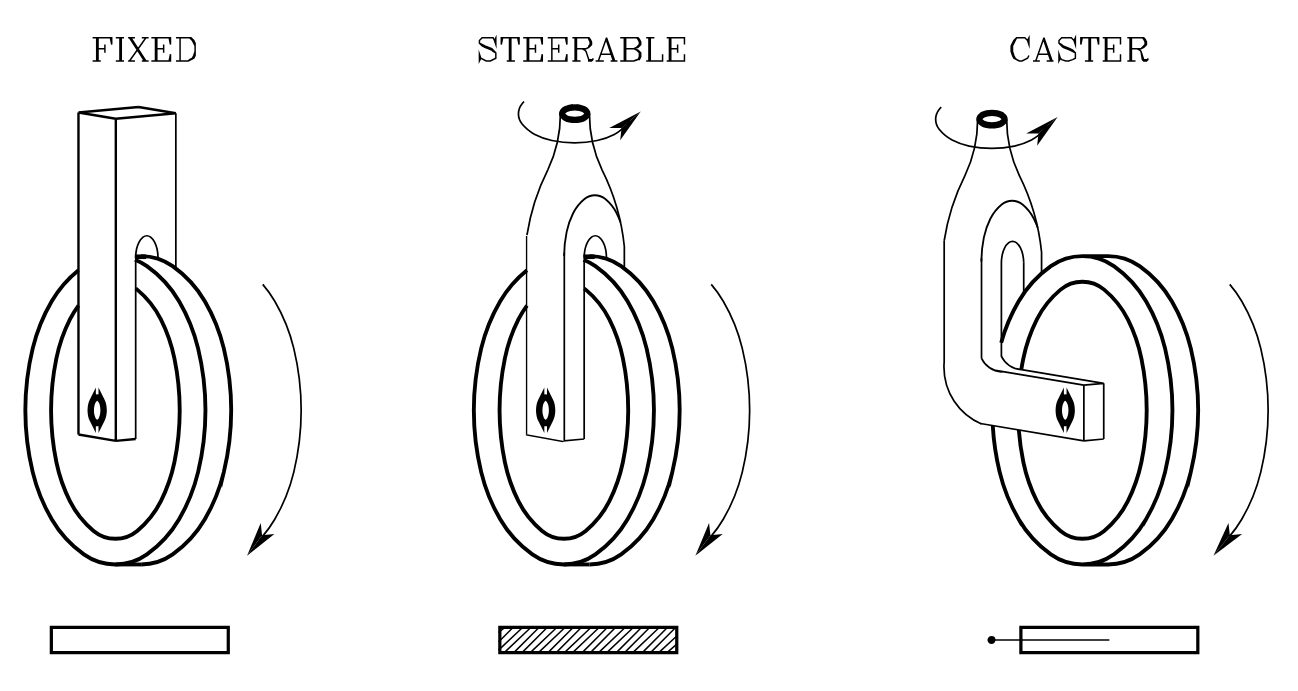
\includegraphics[width=150mm, keepaspectratio]{figures/021_wheels.png}
    \caption{Kerék mechanizmusok \cite{siciliano2010robotics}}
    \label{fig:wheels}
\end{figure}

\begin{itemize}
    \item \emph{Fix kerekek (fixed)}: csak irányban forognak (előre-hátra), nem képesek elfordulni oldalirányban. Általában meghajtott kerekek tartoznak ide, amelyek a robot hajtását biztosítják, például egy autó hátsó tengelyére szerelt kerekek. A robot bázisához mereven csatlakoznak és saját tengelyük körül forognak, amely ortogonális a kerék síkjára.\cite{siciliano2010robotics}
    \item \emph{Kormányozható (steerable) kerekek}: oldalirányban elfordíthatók, a haladási irányuk megváltoztatható, például autó első tengelyén lévő kerekek. A robot bázisához egy csuklóval csatlakoznak, mely lehetővé teszi a kerekek elfordulását, illetve erre merőleges saját tengellyel rendelkeznek (szintén merőleges a kerék síkjára), melyek körül forognak.\cite{siciliano2010robotics}
    \item \emph{Szabadonfutó (bolygó/caster) kerekek}: hasonló mechanikai csatlakozással rendelkeznek, mint az irányítható kerekek, azonban a robot bázisához való csatlakozásuknál található tengely körül szabadon fordulnak el, például irodai székek vagy bevásárló kocsi kerekei. A vertikális tengely nem metszi a kerék elfordulási tengelyét hanem egy "offset" távolságra helyezkedik el. Ezek a kerekek mechanikai stabilitásban segítik a robot bázist.\cite{siciliano2010robotics}
\end{itemize}

\subsection{Mobil kerekes robotok kinematikai modellje}
Kétféle csoportosítás különíthető el: holonomikus (nem tud mozogni a sík bármelyik irányában) és omnidirekcionális (tetszőleges irányba képes mozogni). Omnidirekcionális robotok mecanum (másik nevén svéd) kerekekkel (\refstruc{fig:023_omni_wheel}) felszerelt robotok, melyek több forgó alkatrésszel rendelkeznek, a kerék kerületen mentén független elfordulni képes görgők vannak amik segítségével oldalazó mozgást is végezhet a kerék tengelyével párhuzamosan. \cite{siciliano2010robotics} \cite{ros2_control_docs}

\begin{figure}[!ht]
    \centering
    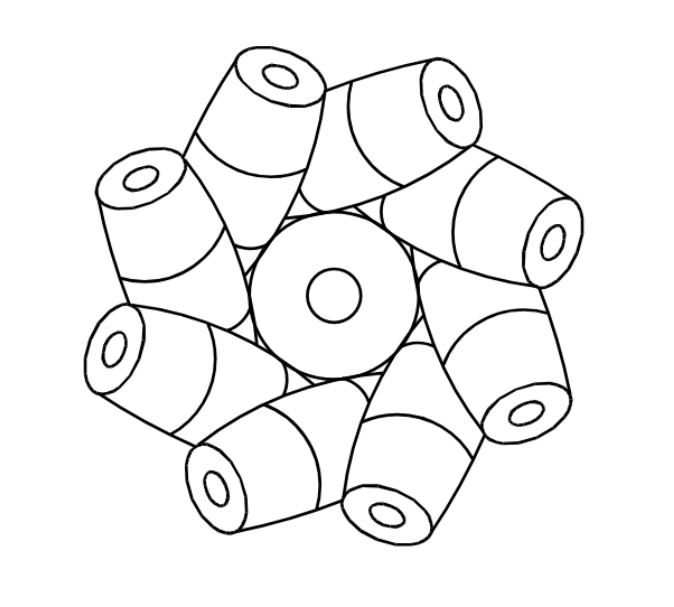
\includegraphics[width=75mm, keepaspectratio]{figures/023_omni_wheel.png}
    \caption{Mecanum kerék \cite{siciliano2010robotics}}
    \label{fig:023_omni_wheel}
\end{figure}

A dolgozatban vizsgált robotmodellek holonomikusak. Több fajta (előző pontban tárgyalt) kerék elrendezéssel hozható létre ilyen robotmodell. Klasszikusan a tricikli modell (\refstruc{fig:024_tricikli_car}), amely egy tengelyen két együttesen meghajtott kerékkel rendelkezik és egy kormányzott kerékkel. Az autókhoz hasonló modellek négy kerékkel (\refstruc{fig:024_tricikli_car}) ahol ebből kettő meghajtott és kettő kormányozható, vagy kettő egyszerre kormányozható és meghajtott plusz kettő stabilitásban asszisztáló fix kerékkel. Differenciál hajtású mobil robotok (\refstruc{fig:025_diff_model}) is a holonomikus robotok közé tartoznak, melyek két függetlenül meghajtott kerékkel és egy vagy több szabadon elforduló kerékkel szerelnek fel.  \cite{siciliano2010robotics} \cite{ros2_control_docs}

\begin{figure}[!ht]
    \centering
    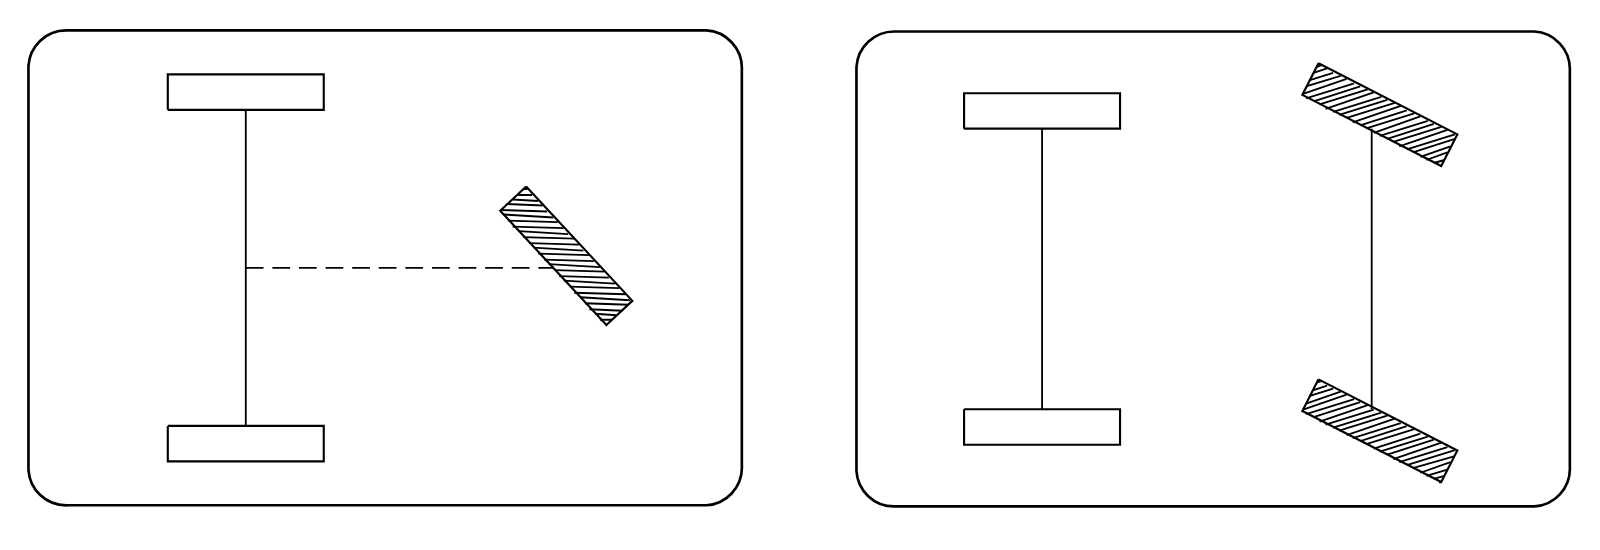
\includegraphics[width=150mm, keepaspectratio]{figures/024_tricikli_car.png}
    \caption{Tricikli és autó modellek \cite{siciliano2010robotics}}
    \label{fig:024_tricikli_car}
\end{figure}

\subsection{Differenciál hajtású robotok}
TODO: források
% Siegwart, R., Nourbakhsh, I. R., & Scaramuzza, D. (2011). Introduction to Autonomous Mobile Robots. MIT Press.
% Bekey, G. A. (2005). Autonomous Robots: From Biological Inspiration to Implementation and Control. MIT Press.

A diplomamunka során használt robotok közül mindegyik ebbe a kategóriába esik. Két szeparáltan meghajtott kerekének köszönhetően egyhelyben képesek megfordulni. A forgás tengelye a két kerék tengelyének közzéppontja. A passzív caster kerék vagy kerekek a stabilitásban segítenek, ezek lekövetik a robot mozgását. Ugye egy sík három pontból már felírható ezért a robot statikai egyensúlya nem jelent problémát, amíg a tömegközéppont vetülete a mozgás síkjára a három vagy több kerek talajjal való találkozási pontjainak egyenes szakaszokkal összekötő polinom belsejében marad. Mint mobil robot a differenciál hajtású szerkezetek munkatere virtuálisan végtelen, ha a munkateret a környezet egy altereként értelmezzük. A valóságban természetesen előjönnek olyan korlátok, mint a robot fizikai kiterjedése és a környezetben lévő akadályok relatív mérete és pozíciója. Természetesen itt sík felületet feltételezve (és kizárva lépcsőket, lifteket stb.) Mint nem omnidirekcionális robotmodell a lokális elmozdulására esnek korlátok. Nem tud rögtön a hajtott kerekek tengelyére merőleges irányába elmozdulni, ehhez szükséges fordulnia. De képesnek tekinthető bármely pozíciót felvenni csak nem rögtön. Ez úgy is kifejezhető, hogy a robot szabadsági fokainak száma alacsonyabb, mint a pozíciót leíró vektor változói. \cite{siciliano2010robotics} \cite{ros2_control_docs}

\begin{figure}[!ht]
    \centering
    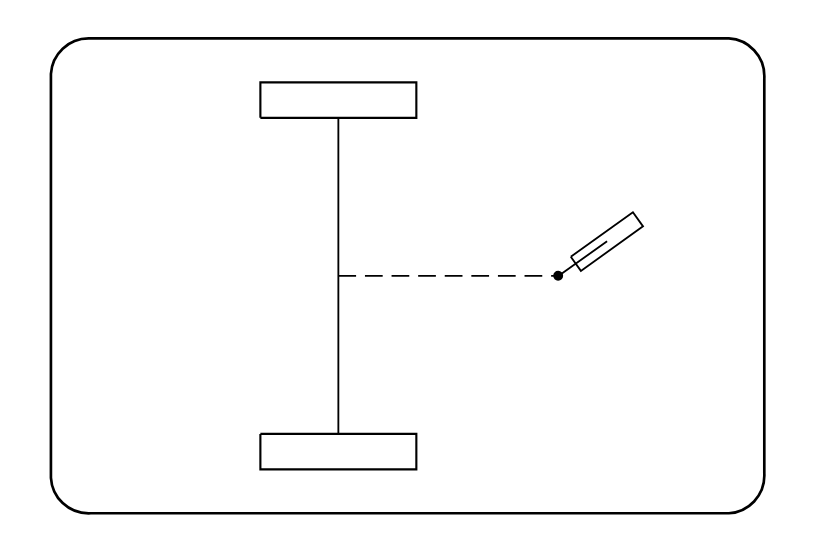
\includegraphics[width=75mm, keepaspectratio]{figures/025_diff_model.png}
    \caption{Differenciál hajtású robot modell \cite{siciliano2010robotics}}
    \label{fig:025_diff_model}
\end{figure}

A differenciál hajtású robotok számos előnnyel rendelkeznek más mechanikai felépítésekkel szemben, amelyek közül az egyik legkiemelkedőbb a szerkezet egyszerűsége. A két különálló hajtott kerék és a passzív támasztó kerekek kombinációja mechanikailag egyszerű és költséghatékony megoldást kínál, amely csökkenti mind a gyártási, mind a karbantartási költségeket. Ez a kialakítás különösen előnyös az oktatási és kutatási célú alkalmazásokban, ahol a költséghatékonyság kiemelt szempont.

Ezen kívül a differenciál hajtású robotok manőverezési képességei kimagaslóak. A két hajtott kerék lehetővé teszi, hogy a robot helyben forduljon, azaz nulla sugarú fordulást hajtson végre, ami rendkívül hasznos szűk helyeken történő navigáció során. Ez a képesség különösen beltéri környezetben, például raktárakban, laboratóriumokban vagy otthoni robotikai alkalmazásokban biztosít jelentős előnyt.

Energiafelhasználásuk szintén kedvező. A differenciál hajtású rendszerek egyszerű hajtásmechanizmusa kevésbé energiaigényes, mint a komplexebb robotmechanizmusok, például a lánctalpas vagy az omnidirekcionális rendszerek. Emellett stabilitásuk is kiemelkedő: a három vagy több támasztópont miatt a robot mozgása stabil, feltéve, hogy a súlypontja a támasztópontok által határolt területen belül helyezkedik el.

Ugyanakkor vannak hátrányai is ezeknek a rendszereknek, különösen más, fejlettebb mechanizmusokkal összehasonlítva. A differenciál hajtású robotok nem omnidirekcionálisak, azaz nem képesek azonnal bármely irányba mozogni. Mozgásuk gyakran több lépést igényel, mivel a hajtott kerekek tengelyére merőleges irányú elmozduláshoz először el kell fordulniuk. Ez korlátozza mobilitásukat dinamikus és változó környezetekben, ahol gyors irányváltásokra van szükség. Ez kihívást nyújt különböző szabályzók tervezésekor, használatakor.

Ezenkívül a differenciál hajtású robotok mozgása sík terephez kötött, ami akadályokkal vagy egyenetlen talajjal tarkított környezetben problémát jelenthet. Fizikai korlátok akadályozhatják nehezebb tárgyak szállításában, szemben például a lánctalpas robotokkal. Továbbá, csúszós felületeken, például koszos vagy nedves padlón, fordulás közben a kerekek megcsúszhatnak, ami pontatlan manőverezést eredményezhet. Ezek olyan problémák, amik kezelhetőek, de fontos megjegyezni, hogy el nem hanyagolhatók. Például nehezebb terhek szállításánál a kerekek terhelése nőhet, ezért opcióként kell tekinteni több bolgyó kerék beépítésére. A talaj és hajtott kerekek közötti súrlódás növelése érdekében a kerekek anyagát és mintázatát is figyelembe kell venni, illetve nem hanyagolható el a gondolat és igény a szoftveres kerék kicsúszás detektálásra és abból eredő korrigálásra, aminek szintén megvannak a maga eszközei, korlátai.

Összességében a differenciál hajtású robotok egyszerűségük, hatékonyságuk és könnyű kezelhetőségük miatt kiváló választást jelentenek számos alkalmazási területen, azonban érdemes figyelembe venni a mobilitásukból és környezeti korlátaikból adódó hátrányokat is. Egy tipikus példa a TurtleBot\footnote{TurtleBot: \url{https://www.turtlebot.com/}}sorozat, amelynek egyszerű és hatékony kialakítása ideális oktatási célokra és beltéri autonóm navigációra. Diplomamunka során három differenciál hajtású robotmodellt használtam. Ebből kettő TurtleBot hármas szérájából a waffle és burger model és egy méretében nagyobb robotmodellt, melynek fejlesztésén munkahelyemen dolgozok. Ezekre később részletesen kitérek, viszont itt szeretnék egy rövid ismertetést írni a TurtleBot-okról.

TODO: képek (tb3 burger waffle)

A TurtleBot egy alacsony költségű, személyes robotkit, amely nyílt forráskódú szoftverrel érkezik, és kifejezetten oktatási, kutatási, hobbi és prototípusfejlesztési célokra tervezték. A diplomamunkám során a TurtleBot 3-as verzióját használtam, azon belül is a Burger és Waffle modelleket. A TurtleBot 3 célja, hogy jelentősen csökkentse a robotplatform méretét és árát, miközben megőrzi a funkcionalitást és minőséget, valamint lehetőséget biztosítson a bővíthetőségre. A robot platformja rugalmasan alakítható át a mechanikai részek újraszerkesztésével (akár otthoni 3D nyomtatott alkatrészekkel) és különböző szenzorok, mikrovezérlővel vagy elektronika hozzáadásával.

TODO: forrás: TurtleBot Inventors Tell Us Everything About the Robot (IEEE Spectrum, By Evan Ackerman, 26 Mar 2013)
https://spectrum.ieee.org/interview-turtlebot-inventors-tell-us-everything-about-the-robot

\subsection{Differenciál hajtású robotok mozgásegyenletei}
TODO: források
% Roland Siegwart, Illah R. Nourbakhsh, Davide Scaramuzza
% Introduction to Autonomous Mobile Robots
% MIT Press, 2011.
% Autonomous Robots: From Biological Inspiration to Implementation and Control
% MIT Press, 2005.

A differenciál hajtású robotok mozgását a kinematikai modelljük írja le, amely az egyes kerekek sebességének és a robot általános mozgási paramétereinek kapcsolatát adja meg. Ezeket a mozgásegyenleteket arra használjuk, hogy a robot mozgását leírjuk, vagy vezérlési parancsokat generáljunk a kívánt mozgás eléréséhez. A mozgásegyenletek alapja, hogy a robot egy síkon mozog, két hajtott kerékkel és esetleg további szabadonfutó kerekekkel van felszerelve.

\begin{figure}[!ht]
    \centering
    \includesvg[scale=1.2]{figures/022_diff_drive.svg}
    \caption{Differenciál hajtású robot 2 dimenzióban \cite{ros2_control_docs}}
    \label{fig:022_diff_drive}
\end{figure}

A \refstruc{fig:022_diff_drive} jelölései a következők. A $v_{right}$ és $v_{left}$ a jobb, illetve bal oldali kerék kerületi lineáris sebessége. Ez a sebesség a kerék érintkezési pontján mért, a kerék síkjára merőleges érintőirányú sebesség, amely meghatározza, hogy a kerék milyen gyorsan halad előre (vagy hátra) a talajon. Az SI mértékegységük $\mathrm{m/s}$. A kerületi sebességek ($v_{right}$ és $v_{left}$) közvetlenül kapcsolódnak a kerék forgási sebességéhez, valamint a kerék sugarához az összefüggés $v = \omega r$ alapján, ahol $\omega$ a forgási sebesség (kerekeké), $r$ pedig a kerék sugara. $v_x$: a robot bázispontjának lineáris sebessége a robot $x$ tengelye mentén. Ez a robot középpontjára vonatkozó előrehaladási sebesség, amely a két kerék sebességének átlaga alapján számítható ki. Az SI mértékegysége $\mathrm{m/s}$.
$\omega_z$: a robot szögsebessége a $z$ tengely körül (amely a síkból felfele mutat). Ez a robot forgási sebessége, amely a két kerék közötti sebességkülönbségen alapul. Az SI mértékegysége $\mathrm{rad/s}$. $w$: a két hajtott kerék tengelyei közötti távolság (nyomtáv). Ez egy statikus paraméter, amely a robot mechanikai kialakításától függ. Az SI mértékegysége $\mathrm{m}$. Ezek a változók szolgálnak a robot aktuális mozgásának modellezésére. S az alábbi mozgásegyenletekkel írják le a robot mozgását:
\begin{align}
    v_{x}      & = \frac{v_{right} + v_{left}}{2}, \\
    \omega_{z} & = \frac{v_{right} - v_{left}}{w}, \\
    v_{left}   & = v_{x} - \omega_{z} \frac{w}{2}, \\
    v_{right}  & = v_{x} + \omega_{z} \frac{w}{2}.
\end{align}

Az egyenletek értelmezése alapján $v_{left}$ és $v_{right}$ a bal és jobb oldali hajtott kerekek sebessége, amelyek a robot általános mozgásának eléréséhez szükségesek. Az egyenletek tehát lehetővé teszik a robot aktuális mozgásának leírását, valamint a kívánt mozgási paraméterek alapján a keréksebességek kiszámítását. Ezek az összefüggések elengedhetetlenek a robot vezérléséhez és navigációjához, valamint az autonóm mozgás tervezéséhez. A diplomamunka során használt robotok irányítása az $v_x$ és $\omega_z$ paraméterek segítségével oldaható meg. A szablyzónak ezeket az értékeket szükséges meghatározni, a mozgásegyenletek segítségével pedig a motorvezérlő vagy szimulációban differenciál hajtást biztosító pluigin feladatkörébe tartozik az egyes kerekek megfelelő sebességének ($v_{right}$ és $v_{left}$) beállítása.

\section{Robotok szabályozása}
A szabályozás kulcsfontosságú a mobil robotok működésében, mivel biztosítja a robot mozgásának stabilitását és pontosságát. Egy autonóm robotnak képesnek kell lennie arra, hogy különböző környezeti feltételek között is megbízhatóan navigáljon, miközben leköveti a kívánt pályát. A szabályozás feladata, hogy a robot kerekének sebességét és irányát dinamikusan módosítsa a kívánt mozgás eléréséhez. Az optimális szabályozás nélkül a robot mozgása instabillá válhat, például csúszás vagy pontatlan kanyarodás léphet fel. Egy jól működő szabályozási rendszer képes kompenzálni a szenzorokból és aktuátorokból származó hibákat, például a kerékcsúszást vagy a zajos pozícióadatokat. A differenciál hajtású robotok esetében a szabályozás különösen fontos, mivel a két hajtott kerék sebességének összehangolása határozza meg a haladási és forgási mozgásokat. A szabályozás lehetővé teszi a robot számára, hogy gyorsan reagáljon a környezet változásaira, például mozgó akadályok elkerülésére. Emellett a szabályozás biztosítja a robot energiahatékonyságát, optimalizálva a hajtáshoz szükséges erőforrásokat. A komplexabb környezetekben, például dinamikus akadályok vagy szűk helyek esetén, a szabályozási algoritmusok teszik lehetővé a robot biztonságos és precíz működését.

Különféle feladatkörök és igények különíthetők el egy autonóm navigáló robot esetében, melyek szétosztása nem a legtriviálisabb feladat, ilyenek lehetnek például a következők:
\begin{itemize}
    \item \textbf{Pályatervezés:} Két pont közötti legrövidebb és legbiztonságosabb (akadályok elkerülése szempontjából) útvonal meghatározása.
    \item \textbf{Pálya követés:} A robotnak a meghatározott pályán való haladásának biztosítása.
    \item \textbf{Kinematikai és dinamikai korlátok betartása:} A robot mozgásának sebesség vagy gyorsulás korlátok között tartása.
    \item \textbf{Akadályok elkerülése:} Dinamikus és statikus akadályok felismerése és kikerülése a mozgás során.
    \item \textbf{Valós idejű döntéshozatal:} A változó környezetben gyors és helyes döntések meghozatala a navigáció során.
    \item \textbf{Hibaelhárítás:} Hibás szenzoradatok vagy váratlan környezeti hatások kezelése, hogy a robot továbbra is folytathassa a feladatát.
\end{itemize}

Ezen feladatkörök többféle alrendszerben különülhetnek el. Tervezési kérdés, hogy melyikért mi felel.
A pályatervezés legtöbbször egy globális tervező feladata, amely az egész mozgástartományról készített reprezentációval dolgozik.

\section{Model prediktív szabályozás}
\section{MPPI}
- különbséges, hasonlóságok
- képeletek
\section{}
\section{Robot Operating System 2 (ROS 2)}
A ROS (Robot Operating System) egy nyílt forráskódú middleware, robotikai keretrendszer. Nem teljes értékű operációs rendszer, ahogy a nevéből gondolni lehetne, hanem a robotfejlesztéshez szükséges szoftverkeretrendszerek halmaza. A munkám során ROS 2 Humble verzióját használtam, ezért a fejezetben a ROS 2 funkcióit és koncepciót ennek a verziónak megfelelően mutatom be. \cite{ros2} \cite{ros2_article}

A ROS 2 egy továbbfejlesztett változata a ROS-nak, amelyet a modern robotika követelményeinek figyelembevételével terveztek újra. a Főbb különbségei közé tartozik a valós idejű működés támogatása, a jobb biztonsági és több szálú működés képességei, valamint a DDS (Data Distribution Service) használata a belső üzenetküldéshez, kommunikációhoz. Míg a ROS 1 a Master-Slave architektúrát használja, addig a ROS 2 a Data Distribution Service (DDS) rendszert alkalmazza, amely nagyobb megbízhatóságot, alacsonyabb késleltetést és jobb skálázhatóságot kínál. A DDS elosztott jellege lehetővé teszi a kommunikációs hibák minimalizálását, valamint támogatja a valós idejű rendszereket. Továbbá, míg a ROS 1-ben két külön könyvtár (roscpp és rospy) létezett, addig a ROS 2 központi, C nyelven íródott rcl könyvtárat használ, amely több programozási nyelvet is támogat, például Python, C++, Java és C\#. A ROS 2 ezenkívül jelentős fejlődést hozott az adatformátum kezelésében is, amely több rugalmasságot kínál a szerializálás terén a belső folyamatok kommunikációjában. A ROS 2 új funkciói közé tartozik a QoS (Minőségbiztosítás) támogatása. Ez magában foglalja az üzenetek megbízhatóságára, határidejére és prioritására vonatkozó beállításokat, amelyek biztosíthatják, hogy a kritikus üzenetek időben kézbesítésre kerüljenek. A többszálú végrehajtás lehetősége node-ok és azok belső folyamatainek párhuzamos futását teszi lehetővé. így jobban ki tudja használni a modern többmagos processzorokat, mint a ROS 1. Mindezek hozzájárulnak a valós idejű feldolgozás javításához, így sokkal jobban alkalmas a komplex, ipari robotikai alkalmazások számára. \cite{ros2} \cite{ros2_article}

Nem célom kitérni és bemutatni teljes végletében a ROS 2 alapelveit és működését, továbbiakban a diplomamunka szempontjából lényeges funckiók, koncepciók kerülnek csak kiemelésre és tárgyalásra, a többi információ a hivatalos dokumentációban megtalálható.

\subsection{Modularitás és node-ok}
ROS 2 olyan szolgáltatásokat, eszközöket nyújt, amelyek lehetővé teszik különböző számítógépekből álló rendszer hatékony együttes működtetését. Ezek közé tartozik az absztrakt hardver kezelés, rengeteg gyártó nyújt a termékükhöz (pl. szenzorokhoz, aktuátorokhoz, vagy akár teljes robotkarokhoz) ROS 2-es csomagokat és támogatást fizikai eszközhöz, gyakran szimulációs környezethez. Nyílt forráskodú, mely hozzájárul a fejlesztők közzötti együttműködéshez, a fejlesztési idő csökkentéséhez, a szoftverek újrafelhasználásához, a szabványosításhoz és a széles körű támogatáshoz. A ROS 2 alapvető építőelemei a node-ok, amelyek az alkalmazások különálló, moduláris komponensei. Minden node egy adott vagy akár több feladatot lát el, például szenzoradatok feldolgozását, mozgástervezést vagy robotvezérlést, és önállóan, más node-októl függetlenül működik. A node-ok egymással üzenetküldés útján kommunikálnak, amely lehetővé teszi az adatok hatékony megosztását, akár különböző számítógépek között is. Több kommunikációs metódus megvólsítható node-ok között, de a lényeg, hogy szabványosított működésüknek köszönhetően már elkészített, mások által lefejlesztett csomagok egyszrűen és viszonylag költségmentesen bővíthetőek saját fejlesztésű node-okkal. A ROS 2 megosztott architektúrája miatt a node-ok nem igényelnek központi vezérlést, ami növeli a rendszer robusztusságát és skálázhatóságát. Ezzel a koncepcióval a node-ok egyszerűen cserélhetők vagy újrahasznosíthatók, megkönnyítve a komplex robotikai rendszerek fejlesztését és bővítését. Egy node leprogramozásakoz a megfelelő nyelvspecifikus könyvtár node osztály implementációjából származtatjuk az osztályt, amely az objektum orientált programozás elveihez kötve örökli az interfészek, paraméterek, időzítők létrehozását. \cite{ros2}

\subsection{ROS 2 client library: rclpy}
Több kliens programkönyvtárat (client library-t) kínál a ROS 2, amelyek lehetővé teszik a fejlesztők számára a ROS 2 rendszerrel való kommunikációt. Több nyelven biztosít klienskönyvtárat, például a kettő legelterjedtebb: C++, Python. Fejlesztői döntés alapján választható, hogy melyi megfelelőbb egy felhasználói esetre. Ha egy gyors és hatékony megoldásra van szükség, akkor egyértelműen a C++-os klienskönyvtár a megfelelő választás, ha viszont a fejlesztési idő csökkentése és a könnyű használhatóság a cél, akár egy adatvizualizációs vagy fájlkezelési problémára, akkor a Python klienskönyvtár a megfelelő választás.

\begin{figure}[!ht]
    \centering
    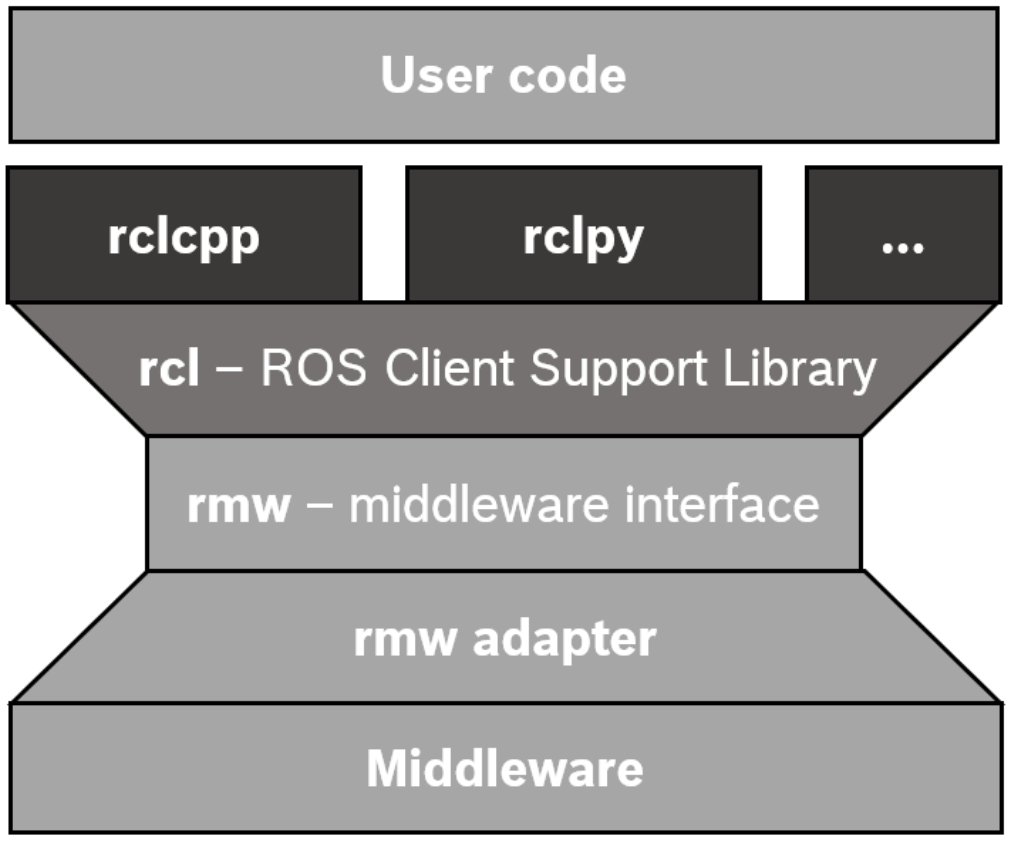
\includegraphics[width=75mm, keepaspectratio]{figures/031_rclpy.png}
    \caption{Client library arhitektúra \cite{ros2}}
    \label{fig:031_rclpy}
\end{figure}

A Python nyelvhez a rclpy csomagot használtam, amely a ROS 2 Python klienskönyvtára. Az rcl C-ben írodott API alapjaira épül és natív Python-os adatstruktúrákat használ. Külön Python kódot generál mindegy egyes ROS 2 üzenet típushoz és az ezekből létrehozott objektumokat fordítja C nyelvre, ha tovább kell küldenie az rcl rétegnek, adattovábbítás céljából. A rclpy csomag, mint client library, lehetővé teszi a Python programok számára, hogy kommunikáljanak a ROS 2 rendszerrel (\refstruc{fig:031_rclpy}), például node-okat hozzanak létre, üzeneteket publikáljanak és feliratkozzanak, szolgáltatásokat hozzanak létre, paramétereket kezeljenek, módosítsanak, szimulációs időhöz férjenek hozzá. Biztosítja a logging lehetőségét és szálkezelési modellt. \cite{ros2}

\subsection{Launch fájlok}
A ROS 2-es launch rendszer célja, hogy a felhasználó számára átláthatóvá tegye és összefoglalja node-ok indítását, paraméterezését és konfigurálását. Ezen kívül a rendszer figyelemmel kíséri (összeszedet logolást biztosít) és esetlegesen reagál a változásokra. A nagyobb rendszerek konfigurációja összetett lehet, ezért a launch rendszer egyik fő előnye a moduláris konfigurációk és az al újrafelhasználhatóság támogatása. Úgynevezett launch fileok írhatóak XML vagy Python nyelven. Lehetőséget biztosítanak az indítási paraméterek meghatározására (TODO: késsőbiekben részletesen), namespace-ek létrehozására (node-ok és paraméterek elkülönítése céljából), interfészek csoportosítására illetve remapping-ek készítésére (topic-ok és service-ek nevének megváltoztatására). Launch argumentumok azaz launch fájloknak megadható paraméterek (nem node paraméterek) definiálhatóak, amikből akár feltételes node indítást lehet leprogramozni, vagy különböző konfigurációk betöltése vezérelhető vagy fájlok elérési útvonala változtatható meg. Launch fájlok segítségével tehát egyszerre indítható és állítható le több node. Futás közben monitorozható és futás után log fájl megtekintésével debugolható. Rengeteg előnyt biztosítanak tehát a launch fájlok. Ebben az összefoglalóban szintén a részletekre nem, csak a munka szmepontjából lényeges tulajdonságokra tértem ki. \cite{ros2} \cite{ros2_design}

\subsection{Interfészek}
A ROS 2 alkalmazások, node-ok jellemzően háromféle interfész típuson keresztül kommunikálnak: messages, services, és actions. Ezek leírására a ROS 2 egy egyszerűsített interfészleíró nyelvet (IDL) használ, amely megkönnyíti az interfész típusának forráskód-generálását több programozási nyelvre. Az IDL lehetővé teszi, hogy az interfészek adattípusai egyszer legyenek megírva szabványosított formátumban és az ezekből generált különböző nyelvű forráskód autómatikusan történjen. Minden node-nak lehet több különböző interfésze és típusunkont és bármennyi.

A publisher-subscriber kommunikációs modell a .msg típust használja. A publisher adatok továbbítására szolgál egy topic-ra, amelyet a subscriber olvas. Egy topic-ra több publisher és több subscriber is csatlakozhat, ebben az esetben mindegy egyes subscriber megkapja az üzenetet. A service-k a .srv típust használják, amely egy kérést (request) és egy választ (response) tartalmaz. A kliens küld egy kérést a szolgáltatásnak, amely válaszol a kérésre. Az action-ök a .action típust használják, amely egy kérést (goal), egy visszajelzést (feedback) és egy választ (result) tartalmaz. Az action-ök a service-ekhez hasonlóan működnek (szintén kliens-szerver modell), de megszakíthatóak és visszajelzést adnak a kliensnek a folyamat állapotáról. \cite{ros2} \cite{ros2_design}

\subsection{Paraméterek}
A paraméterek a ROS 2-ben eredendően node-okhoz kapcsolódnak. Egy node létrehozásakor definiálhatunk paramétereket, melyekkel a node futásához szükséges adatokat tárolhatunk. Ennek az implementációnak előnye, hogy modularitás és skálázhatóság elvét segíti, azaz különböző felhasználó igényeknek könnyen átszabhatóvá teszi a node-okat. Például egy szabályzó frekvenciája definiálható ilyen paraméterként, s ezáltal állíthatóvá válik különböző futás körülmények között. A paraméterek a ROS 2 node-okhoz kapcsolódnak, és azok konfigurálására szolgálnak az indításkor vagy futás közben, anélkül hogy a kódot módosítani kellene. Egy paraméter élettartama szorosan kapcsolódik a node-éhez, bár a node implementálhat olyan mechanizmusokat, amelyek az értékeket újra betöltik egy újraindítás után. Minden paraméter egy kulcsból, egy értékből és egy típusból áll, az érték különböző típusokat vehet fel. Részletesen a hivatalos dokumentációban elérhetőek a különböző típusok, amit lényeges megemlíteni, hogy a paraméterhez tartozó definit típus meggátolja, hogy futási időben a meghibásodás lehetőségét. A paraméterek nevét, típusát szükséges a node implementációjában megszabni. Az értéke opcionálisan megadható, illetve lehetőség van alapértelmezett érték megadására is. A paramétereket a node-ok indításakor is megadhatóak parancssoron, vagy node-ok launch fájlból indításakor kódból, vagy .yaml fájlból is. A paraméterek felülírhatók, tehát előre definiált alapértelmezett értéküknél egyel magasabb fokon van a launch fájl és a node "ros2 run ..." parancsal indításakor megadott érték. Ez mellett a launch fájlokban beimportált .yaml configurációs fájlokkal is felülírhatók. A .yaml fájlok nagy előnye, hogy sok paraméter esetén átláthatóbbá teszi a konfigurációt, könnyen módosítható és újrahasználható. Ugyanis egy konfigurációs fájl több node paraméterét is tárolhatja.

A paraméterek hatalmas előnye, hogy lehetőséget biztosítanak futás közbeni módosításra.  A node paramétereit futás közben API-n keresztül, vagy külső folyamatokból paraméter service-ekkel lehet módosítani. A paraméterek változását "set parameter callback" vagy "on parameter callback" függvények segítségével előre definiálni kell. Ha egyszerű értékadás történik akkor is. Ennek az az előnye, hogy olyan paraméter megváltoztatása esetén, ha olyan változik amely kihatással van a működésre (pl. frekvencia, időzítők periódusideje vagy szabályzó paraméterek) leprogramozható mi történjen a hatására. Interakcióba a paraméterekkel különféle módokon juthatunk. Egyik módja parancsoros eszköz használata a "ros2 param set/get/..." szolgáltatás, mellyel változtatni illetve értéket lekérni is tudunk. Ha autómatizálni szeretnénk, amely a diplomamunka egy fő motívuma, egy másik futó node-ból service hívással is megtehető. Minden node-hoz tartoznek service-ek amik lehetővé teszik a futás közbeni érték cserét. \cite{ros2} \cite{ros2_design}

\subsection{Executors}
TODO: kép
Az executor-ok menedzselik ROS 2-es folyamatok végrehajtását. Az executor egy olyan entitás, amely felelős a node-ok futtatásáért és események (időzítő vagy üzenet érkezés) hatására kiváltott callback-ek végrehajtásáért. Az executor-ok lehetővé teszik a node-ok párhuzamos futását. Az executorok az alap operációs rendszeren keresztül a processzor szálait használják a folyamatok futtatására. Az executor felelős a megfelelő függvények meghívásáért üzenetek vagy események feldolgozása céljából. Ellentétben a ROS 1-el, ahol a beérkező üzeneteket a klienskönyvtár szintjén tárolták sorban, a ROS 2-ben az üzenetek a köztes rétegben (rcl) maradnak, amíg a függvények feldolgozzák őket. Ez a tervezési megközelítés összhangban van a szolgáltatás minőséget biztosító (QoS) szabályokkal, biztosítva az erőforrások hatékonyabb kezelését. Az executor-ok "wait set" mechanizmust használnak a rendelkezésre álló üzenetek figyelésére és az időzítők lejártának észlelésére, így optimalizálva a visszahívások kezelését. A ROS 2 háromféle executort kínál, amelyek eltérő felhasználási esetekre vannak szabva. \cite{ros2} \cite{ros2_design}

\begin{itemize}
    \item \emph{Egyszálas executor (Single-Threaded Executor)} a legegyszerűbb executor, amely egyetlen szálat használ a függvényhívások sorozatos feldolgozására. Olyan node-okhoz ideális, ahol a párhuzamos futás nem szükséges vagy nem kívánatos. \cite{ros2}

    \item \emph{Többszálas executor (Multi-Threaded Executor)} a párhuzamosságot szem előtt tartva több szálat használ a visszahívások egyidejű feldolgozására. A szálak száma konfigurálható, lehetővé téve a teljesítmény jelentős növelését olyan rendszerekben, ahol nagy a függvényhívások száma terheli a rendszert vagy az alacsony késleltetés kritikus szempont. A párhuzamos feldolgozást a callback csoportok logikai szabályai határozzák meg. A callback csoportok abból a szempontból lényegesek, hogy ezek segítségével tudja értelmezni a folyamatok prioritását. Kétféle csoport létezik: a "Mutually exclusive", mely elemei nem futhatnak párhuzamosan és a "Reentrant", mely elemei párhuzamosan futtathatóak. Külöböző callback cosportokhoz tartozó folyamatok lefuthatnak párhuzamosan. Ennek nagy szerepe az adatok feldolgozásánál van, segítségükkel megakadályozhatók a versenyhelyzetek és a deadlock-ok. \cite{ros2}

    \item \emph{Statikus egyszálas executor (Static Single-Threaded Executor)} optimalizálja azokat az eseteket, ahol a node-ok szerkezete (pl. subcriber-ek, időzítők) nem változik a futásidő során. Csak egyszer vizsgálja meg a node felépítését az inicializáláskor, szemben a másik két executor-ral, amelyek rendszeresen újravizsgálják azt. Ezért a statikus egyszálas executor-okat csak olyan node-ok esetében ajánlott használni, amelyek minden szükséges komponenst az inicializálás során hoznak létre. \cite{ros2}
\end{itemize}

\subsection{Composition}
A composition egy olyan koncepció amely megbontja a modularitását a ROS 2-es rendszernek. Teszi ezt azért, hogy gyorsabb feldolgozást nyerjen. A megszokott külön node-okban külön folyamatok helyett a node-okat lehetőség van átalakítani és "component"-ként regisztrálni, majd többet egy "container"-be betölteni. Így külön "process"-ek helyett egyben futnak. Ezt a koncepciót azért szükséges kiemelni, mert a NAV2 használja. A composion-nel megvalósíthat az "intra-process communication" (IPC), aminek lényege, hogy ugyanazokat az adatokat használó node-ok nem üzenetekkel kommunikálnak, hanem gyakorlatilag memóriacímekkel. Tehát egy container-ben indított két node ha ugyanahhoz az adathoz akar hozzáférni, a szoksásos interface-eken keresztül megteheti viszont csak virtuálisan lesz az üzenetként elküldve. Ez helyett például egy kép feldolgozó "pipeline" működésénél az adott kép memóriába töltése után a két node ugyanúgy éri el, közöttük a a kommunikáció közvetlen memóriaozáféréssel valósul meg, így gyorsítva a feldolgozást és csökkentve az erőforrás igényt. Mivel process-ek közötti kommunikáció sokkal lassabb mint az egy process-en belüli. Az IPC segítségével a különböző folyamatok közötti kommunikáció során csökkenthető az adatmásolások száma. A memóriában elhelyezett adatokat közvetlenül is megoszthatja a rendszer a folyamatok között, minimalizálva a teljesítményveszteséget. Az IPC a zero-copy technikát használhatja, amely lehetővé teszi, hogy az adatokat közvetlenül a memóriában osztják meg a résztvevő folyamatok között, további másolási műveletek nélkül. Ez különösen hasznos, ha nagy méretű üzeneteket (például szenzoradatokat vagy képeket) kell továbbítani. Mintilyen nagy méretű szenzoradatokkal dolgozo csomag a NAV2 és különböző funkciói jelentősen profitálnak belőle. Előny, hogy nem szükséges manuálisan konfigurálni az adatátvitelt; a ROS 2 maga dönti el, hogy mikor használja az IPC-t a teljesítmény javítása érdekében. Továbbá biztonságtechnikailag is jó döntés lehet, mert helyi környezetben az IPC lehetővé teszi, hogy az adatok ne kerüljenek ki a hálózatra, ezáltal csökkentve a hálózati forgalmat és a kapcsolódó késleltetést. \cite{ros2} \cite{ros2_design}

\section{Gazebo}
A Gazebo egy népszerű nyílt forráskódú szimulációs környezet, amelyet robotikai alkalmazások fejlesztéséhez és teszteléséhez használnak. 3D grafikai megjelenítést, fizikai szimulációt, valamint szenzor- és robot leíró modelleket kínál. Lehetővé teszi, hogy valós világot imitáló környezetekben robotot tesztejünk anélkül, hogy fizikai hardvert kellene használniuk. Támogatja a különböző robotikai központi rendszerek, például a ROS 2 integrációját, így valósághű szimulációt nyújt mind a vezérlés, mind a kommunikáció szempontjából.

TODO: számok mértékegységek

A Gazebo-ban a szimulációs környezetet az úgynevezett world fájlok írják le, amelyek a világ statikus elemeit (például tereptárgyak, falak vagy akadályok) és dinamikus elemeit (pl. robotmodellek, mozgó dinamukis akadályok) definiálják. A világfájlok általában .world kiterjesztéssel rendelkeznek, és az SDF (Simulation Description Format) vagy URDF (Unified Robot Description Format) nyelvet használják a környezet leírására. A szimulációban definiálhatóak a fizikai motor típusa, az alapértelmezett, amit én is használtam az ODE (Open Dynamics Engine). Word fájlokban a fizikai motor kapcsán definiálhatóak azok paraméterei ilyen az ODE esetében a \emph{"max\_step\_size"}, ami a lépésköz időtartamát jelenti. A \emph{"real\_time\_update\_rate"} határozza meg, milyen gyakorisággal halad előre a szimulációs idő lépésenként valós időben. Alapértelmezetten a \emph{"max\_step\_size"} 0.001 másodperc, a \emph{"real\_time\_update\_rate"} pedig 1000 hz, szóval kettőt megszorozva egymással egyet kapunk, ami azt jelenti, hogy a szimuláció, ha a megfelelő erőforrások és számítási kapacitás rendelkezésre áll, valós időnek megfelően halad. \cite{gazebo}

A robotmodelleket a Gazebóban általában URDF, SDF vagy XACRO fájlok segítségével írják le. Egy robotmodell főbb elemei közé tartoznak a "link"-ek és a "joint"-ok. A link-ek a robot fizikai komponenseit, például a testét vagy karjait reprezentálják, míg a joint-ok a link-ek közötti mozgásokat határozzák meg, például forgó vagy csúszó kapcsolatokat. A modellekhez anyagokat és színeket is rendelhetünk, amelyek a vizuális megjelenést adnak. Ezenkívül dinamikus tulajdonságok, például a tömeg, a súrlódás és a tehetetlenségi mátrix is definiálható, amelyek a valósághű fizikai szimulációhoz szükségesek. \cite{gazebo}

A Gazebóban a robotok szenzorokkal szerelhetők fel, amelyek valósághű adatokat szimulálnak a környezetről. A szenzorok, például lézerszkennerek (Lidar), kamerák, inerciális mérőegységek (IMU) vagy GPS, pluginok segítségével integrálhatók a robotmodellbe. Ezek a pluginok definiálják a szenzorok működését, például a látómezőt, a mintavételezési frekvenciát vagy a zajmodelljüket. A szimuláció során a szenzoradatok valós idejű információkat szolgáltatnak, amelyeket a robot vezérlőrendszere felhasználhat például navigációhoz, térképezéshez vagy akadályelkerüléshez. \cite{gazebo}

A ROS 2 és a Gazebo közötti kommunikáció általában topicokon keresztül valósul meg. A Gazebo ROS 2 pluginjai lehetővé teszik, hogy a szimulált robotok ROS 2 node-okként viselkedjenek, amelyek publikálnak vagy feliratkoznak topicokra. Például egy szimulált kamera pluginja képes képkockákat publikálni egy beállított topicra, amelyet egy ROS 2 node dolgozhat fel. Hasonlóképpen, a robot vezérléséhez szükséges parancsok, például sebességparancsok, a Gazebo felé is elküldhetők. Ez a szoros integráció lehetővé teszi, hogy a fejlesztők a szimulált környezetben ugyanazokat az algoritmusokat és vezérlőket használják, mint a valós robotokon, minimalizálva a valós és a szimulált környezet közötti eltéréseket. \cite{gazebo}

\section{Navigation 2 (Nav2)}
A Nav2 (Navigation 2) a ROS 2 navigációs keretrendszere, ROS 2-es csomagok összessége, amely robotok autonóm mozgását teszi lehetővé. Lehetővé teszi a robot számára, hogy egy térképen egy kiindulási pontból egy megadott célponthoz navigáljon, miközben akadályokat kerül ki. A Nav2 különféle algoritmusokat kínál, például útvonaltervezést, térképezést, helymeghatározást és akadályelkerülést. Moduláris felépítésének köszönhetően rugalmasan testreszabható, így különböző robotplatformokon használható. A rendszer főbb komponensei közé tartozik a globális és lokális útvonaltervező, a helymeghatározás (AMCL), valamint a vezérlési algoritmusok, például az MPPI és a DWB. A Nav2 kompatibilis a Gazebo szimulátorral és valós robotokkal egyaránt, és ROS 2 interfészeket, például topic-okat, service-eket és action-öket használ a kommunikációhoz. A fejlesztők széles körben alkalmazhatják beltéri és kültéri navigációs feladatokhoz. \cite{nav2}

A navigációs feladatok központi elemei a útvonal tervezők (planner-ek) és a vezérlők (controller-ek), amelyek a robot mozgásának megtervezését és irányítását végzik. A rendszer hibakezelési képességének biztosítása érdekében helyreállítási mechanizmusokat (recoverie-k) alkalmaznak, amelyek célja a robot kimozdítása egy kedvezőtlen helyzetből vagy különféle problémák kezelése. További útvonal minőségi javítás érdekében az útvonaltervek finomhangolására smoother-ek használhatók. \cite{nav2}

A Nav2 egy kiterjedt nyílt forráskódú szoftvercsomag, amely folyamatosan fejlődik a ROS 2-es közösség hozzájárulásának köszönhetően. Ebben a fejezetben szintén, mint a ez eddeigiekben a Nav2 azon koncepcióira fogok kitérni is bővebben elemezni, melyek a diplomamunka során használtam és fontosak a megértés szempontjából.

\subsection{Costmap}
TODO: kép %https://wiki.ros.org/costmap_2d

A costmap a robot környezetének térbeli reprezentációja, amelyet a navigációs rendszerek használnak az útvonaltervezéshez és mozgásvezérléshez. Ez egy kétdimenziós, szabályos rácsszerkezet (grid), ahol az egyes cellák bizonyos költségeket reprezentálnak, például ismeretlen, szabad, elfoglalt vagy "felfújt" költség értékekkel. A "felfújás" (inflation) folyamata során az akadályokkal elfoglalt cellák költségeit továbbítják a környező cellákba, ahol a költség a távolság növekedésével csökken. Ez lehetővé teszi, hogy a robot elkerülje a veszélyes területeket, miközben figyelembe veszi saját méretét és a felhasználó által megadott preferenciákat, például tiltott vagy kevésbé preferált zónák definiálásával. \cite{ros_wiki}

Egy costmap lehet globális vagy lokális, attól függően, hogy a teljes térképezett környezetet vagy a robot egy lokális környezetét reprezentálja. Általánosan a globális útvonal tervezés a globális costmap-en történik, a dinamikus akadályelkerülés és mozgásszabályozás a lokális costmap-en. A costmap-ek különféle rétegekből állhatnak össze, melyek külön külön a rácspontokat megjelölhetik szabad, foglalt stb. állapotokkal. Majd ezek a rétegek összeadódnak, így kapjuk meg a teljes costmap-et. Rétegek lehetnek statikusak, mondjuk egy előre elkészített térkép reprezentáció a környezetről vagy dinamukusan változó akadályok szenzorok adataiból kinyert és feldolgozott reprezentációi. Ilyen rétegek kezelek 2 vagy 3 dimenziós szenzoradatokat például LIDAR, RADAR, szonár, mélységérzékelők vagy kamerák által gyűjtött adatokat dolgoznak fel, tárolnak és menedzselnek. Ezeket a rétegeket a "pluginlib" segítségével lehet betölteni, implementálni, lehetővé téve a testreszabást és a fejlesztő által szükséges előfeldolgozási lépések integrálását. \cite{nav2}

\subsection{Planner-ek}
A planner-ek elsődleges feladata a robot útvonalának megtervezése egy adott célfunkció teljesítése érdekében. Példák a tipikus tervezési feladatokra: egy adott célt megközelítő útvonal meghatározása, vagy egy teljes terület lefedésére irányuló pálya megtervezése. A Nav2-ben a globális útvonaltervezők (global planners) a robot teljes útvonalát tervezik meg a kiindulási ponttól a célpontig. Egy térképen a környezet szenzorokból nyert adatiból feldolgozott virtuális megjelenítésén terveznek. Többféle algoritmust kínál a Nav2, amelyeket plugin-ként lehet a "planner\_server" node-ba betölteni és akár futásidőben váltani köztük. Az összesnek általános feladatai: legrövidebb út kiszámítása, teljes pálya generálása. Ezek a célok definiálják az optimális pályát általában, de nem kizárólag. A diplomamunkának nem volt célja különböző planner-ek összehasonlítása, ezért az "alap" példaként biztosított NavfnPlanner-t használtam, általánosságban elmondható róla, hogy egy kifejezetten stabil A* vagy Dijkstra opcionálisan konfigurálható algoritmusok valamelyikét használja, robotot alakját körrel közelíti és így tervezi meg a pályát a globális costmap-en. \cite{nav2}

\subsection{Controller-ek}
A vezérlők (controller-ek) a Nav2 rendszerben a robot irányításáért felelős komponensek, amelyek a globálisan kiszámított útvonalak követését vagy lokális feladatok végrehajtását biztosítják. Ezek a Nav2-ben a controller\_server által kerülnek kezelése, amely egy olyan kiszolgáló, amely különböző vezérlési algoritmusokat tartalmazhat plugin formájában.

A controller hozzáfér a helyi környezet reprezentációjához a lokális costmap-en keresztül és megpróbál kinematikailag megvalósítható vezérlési parancsokat előállítani. A controller-ek működése iteratív: egyes algoritmusok a robot aktuális helyzetéből kiindulva, egy előre vetített pályát számolnak minden frissítés során, hogy biztosítsák a lokálisan optimális és megvalósítható irányítást. Az irányítás egy topic-ok jelenik meg, megszokottan a "cmd\_vel" topic-on, ahonnan a robot motor interfészének olvassa, majd továbbítja például a motorok felé. \cite{nav2}

\subsection{Navigator API}
A Nav2 kínál egy "nav2\_simple\_commander" névre hallgató Python könyvtárat, mely gyakorlatilag egy API a Nav2-es rendszerhez, mamin keresztül interakcióba léphetünk az épen futó node-okkal. Ez az API "elrejti" a ROS 2 és a Nav2 komplexitásait, így segítve, hogy kizárólag egy alkalmazás fejlesztésére koncentrálhasson a felhasználó. Biztosítja az összes szükséges funkciót a navigációs rendszer kezeléséhez, miközben lehetőséget ad arra, hogy a fejlesztők saját igényeik szerint konfigurálják a Nav2-t az egyéni pluginjaikkal. Az API függvényei egy szálon futattve nem blokkolnak, ezért végrehajtásuk közben lehetőség van visszajelzések feldolgozására és hibakezelésre. Ez különösen hasznos, amikor a robot mozgása közben valós idejű adatok elemzésére vagy a rendszer vezérlésére van szükség. Támogatja a kiadott utasítások preemptív megszakítását, és feladatok közötti váltáskor az explicit megszakítást. API-n keresztül elérhető funkciók, lényeges, de nem teljes felsorolása: inicializálási pozíció megadása, célpontra navigálás elindítása, navigáció állapotának és eredményének lekérése, útvonal követés indítása, costmap-ekkel való interakció és térképváltoztatás. Ezek-et a funkciókat a diplomamunka során is hanszáltam, működésükről a megértést segítve tervezés/fejlesztés fejezetben később részletesen írok. \cite{nav2}

\subsection{MPPI Nav2-ben}
A Nav2 MPPI Controller (Model Predictive Path Integral Controller) a Nav2 stack prediktív vezérlő algoritmusa, amely a TEB és hagyományos MPC útvonal-követési vezérlők utódjaként jelent meg. Ez egy mintavételezés-alapú megközelítést alkalmaz az optimális pályák kiválasztására, iteratív optimalizálást végezve a vezérlési iterációk között. A vezérlő kiegészíthető és testreszabható plugin-alapú objektívfüggvények segítségével, amelyek különböző viselkedéseket és attribútumokat támogathatnak. Támogatja a differenciális hajtású, omnidirekcionális és Ackermann-kormányzású robotokat. A vezérlő akár 50 Hz-es vagy nagyobb frissítési sebességgel képes futni közepes teljesítményű processzorokon (pl. 4. generációs Intel i5). Nem konvex és nem differenciálható objektívfüggvények támogatása, ami jelentős tervezői rugalmasságot biztosít. Egy modell-alapú prediktív vezérlő (MPC) variáns, amely iteratív megközelítéssel találja meg a robot számára optimális sebességparancsokat. Az algoritmus lépései:

\begin{itemize}
    \item \textbf{Kezdeti állapot:} Az előző időlépés legjobb vezérlési megoldása és a robot aktuális állapota alapján történik a vezérlés.
    \item \textbf{Perturbációk alkalmazása:} Egy Gauss-eloszlásból véletlenszerűen mintavételezett perturbációk kerülnek a vezérlési parancsokra.
    \item \textbf{Szimuláció:} Ezeket a zavarokkal módosított vezérlési parancsokat a robot mozgásmodelljén keresztül előre szimulálja, amely különböző pályákat generál.
    \item \textbf{Pontozás:} A generált pályákat egyedi, plugin-alapú függvények segítségével súlyozza.
    \item \textbf{Vezérlési döntés:} A pályák pontszámait egy softmax függvény segítségével súlyozza, és ennek alapján választja ki az aktuális vezérlési parancsot.
    \item \textbf{Iteráció:} Az optimalizálási folyamatot többször megismétli, amíg a vezérlési parancsok kielégítőek nem lesznek.
\end{itemize}

Az MPPI Controller lehetővé teszi komplex és nem hagyományos viselkedések implementálását, mivel az objektívfüggvények tervezői szabad kezet kapnak a nem konvex és nem differenciálható szabályok használatában. Ez az innovatív megközelítés rugalmasabbá teszi a vezérlőt kutatási és ipari környezetben egyaránt.

\section{Odometria és TF}
Eddig sokszor volt szó a robot pozíciójáról és említve volt, a Gazebo fejezetben, hogyan hozható létre robot modell szenzorokkal. Ezekhez köthető az odometria (odometry) és koordináta-transzformációk rendszere (tf). A különböző koordináta-rendszerek és azok közötti átalakítások biztosítják, hogy a robot megfelelően érzékelje és kövesse a mozgását a környezetében. Három alapvető koordináta-rendszert használ a ROS 2:

"base\_link": A robothoz kötött koordináta rendszer, mely vele együtt mozog. Virtuálisan definiált, tetszőleges pozícióban és orientációban lehet. A robot modell felépítésénél a base\_link koordináta rendszeréhez képest kell definiálni a robotra szerelt szenzorokat és aktuátorokat, vagy a robot testét.

"odom": A világhoz rögzített globális koordináta rendszer. Az odom rendszerben a robot pozíciója idővel eltolódhat, ami miatt hosszú távon nem ideális globális referenciaként. Azonban a robot pozíciója az odom koordináta-rendszerben folytonosan változik, ugrások nélkül. Az odometria a robot relatív elmozdulását jelenti (például kerék-odometria, vizuális odometria vagy inerciális mérési egység) az odom rendszert használja rövid távú lokalizációhoz.

"map": Szintén globális környezethez, világhoz rögzített referencia, amelynek Z-tengelye felfelé mutat. A map koordináta rendszerben a robot pozíciójának nincs összeadódó hibája, mint az odom rendszerben. Viszont nem biztosít folyamatos pozícióváltoztatást, mert a lokalizáció hatására, szenzoradatok frissülése miatt időnként ugrások léphetnek fel a pozíciókban.

A robot navigációjában különböző koordináta-rendszerek között transzformációkra van szükség, hogy biztosítsák a helyes pozicionálást és mozgást. A transzformációk biztosítják a különböző koordináta-rendszerek közötti átváltást, például az odom, base\_link és map rendszerek között. Az transzformációk szükségesek, ha egy szenzor által, saját koordináta rendszerében érzékelt tereptárgyat akarunk a robot koordináta rendszerében elhelyezni, hogy a kikerülés manőverét megtervezzük. A két legfontosabb transzformáció az odom-ot base\_link-kel összekötő és a map-ot az odom-mal összekötő.
TODO(kép map->odom->base\_link). Az előbbit az odometria forrásokból számolt transzformáció adja, az utóbbit aa lokalizációs alrendszer biztosítja. \cite{ros_wiki} \cite{ros2_design}

\section{Lokalizáció - AMCL}
Már sokszor említettem a lokalizációt aminek a szerepe, hogy adott globális koordináta rendszerben elhelyezze a robotot. A diplomamunka során futtatott szimulációkhoz Lidar alapú AMCL (Adaptive Monte Carlo Localization-t) használtam. Az AMCL egy statisztikai alapú lokalizációs algoritmus, amely a robot pozícióját és orientációját becsüli a térkép és a szenzoradatok alapján. Az AMCL a Monte Carlo módszert alkalmazza a robot helyzetének valószínűségi eloszlásának közelítésére, amelyet a szenzoradatok folyamatosan frissítenek. Az algoritmus a robot pozícióját egy többdimenziós Gauss-eloszlásként reprezentálja, amelynek középpontja a becsült helyzet, a szórása pedig a bizonytalanságot jelzi. \cite{nav2}
%----------------------------------------------------------------------------
\chapter{Tervezés}
%----------------------------------------------------------------------------
Ebben a fejezetben kifejezette a tervezés lépéseit és a munka logika felépítését szeretném bemutatni. A cél röviden egy olyan rendszer létrehozása volt ami minimális felhasználói beavatkozásra képes elindítani egy szimulációs környezetet a robotról és méréseket, optimalizációkat futattni.

\section{Probléma felvetés}
A kiindulási pont a munkahelyemen fejlesztett robot, amely ROS 2-őt használ különböző funkciói végrehajtásában. Az egyik alap funkció vagy feladata az autonóm navigáció, amelyet a Nav2 stack-ben lekódolt MPPI szabályzóval valósít meg. A szabályzóhoz különféle crtic függvényeket valósítottak már meg plugin-ok formályában. Ezeknek két jellemző paramétere van: cost\_weight és cost\_power. A ezeknek a kombinációja határozza meg az MPPI által generált bevatkozó sebességekből generált pályák kiértékelését. A két paraméter hangolásával (critic-enként állítható) szabályozható, finomítható a robot viselkedése.

A korábbiakban írtam arról, hogy az autonóm navigációnál különböző feladatkörök milyen módon specifikálhatók és oszthatók szét, jelen esetben a szabályzó elsődleges feladataként a globális útvonaltervező által készített útvonal lekövetését fogalmaztam meg. Másodlagos feladatként a kinematikai korlátok: maximális és minimális sebesség, gyorsulát jelöltem ki. Értelemszerűen szükséges valamilyen határt szabni egy szabályzó feladatkörének, a használt komponensek lehetőségeit tekintve ezek a legkézenfekvőbbek.

Szóval a cél egyértelmű: bizonyos számú critic függvény paraméterének beállítása, hangolása, hogy a szabályzó képes legyen a megjelölt feladatokra. Ehhez szükséges volt egy introspekciós eszköz megtervezése és lefejlesztése, amivel képesek vagyunk monitorozni a szabályzó működését, kiértékelni különböző paraméterek hatását a robot viselkedésére. Definiálni mérhető paramétereket, amelyek alapján az összehasonlítás elvégezhető. Hosszú távú célként megfogalmazásra került, egy olyan rendszer létrehozása, amellyel hangolható autómatikusan a szabályzó paraméterei. Ezt elsősorban szimulációban a legegyszerűbb elvégezni, de a szimuláció és a valóság közötti különbségek miatt a szimulációban kapott eredményeket valós környezetben is ellenőrizni kell, tehát lehetőséget kell hagyni, hogy minimális átalakítással valós fizikai környezetben is használható legyen.

\section{Követelmények}
Egy olyan szoftver csomag létrehozása került a diplomamunka fókuszábam, amely képes a Nav2 stack-ben használt MPPI szabályzó paramétereinek monitorozására, a paraméterek hatásának vizsgálatára. Elsősorban szimulációban. A szoftvernek képesnek kell lennie:
\begin{itemize}
    \item Az eddig használt ROS 2 stack indításának támogatása launch fájlokkal.
    \item Szimulációk futtatásának lehetősége a Gazebo környezetben.
    \item Olyan paraméterek mérésének biztosítása, amelyekből eldönthető a különbség a konfigurációk között.
    \item Megismételhető és dokumentálható mérések végrehajtása, amelyek a mérhető paraméterek megfelelő kompozícióján alapulnak.
    \item A mérések eredményeinek szemléltetése, segítve a fejlesztőket a döntések meghozatalában.
    \item A szimuláció során alkalmazott paraméterek egyszerű módosíthatósága.
    \item Az optimalizáció támogatása, többek között a szimulációk párhuzamosításával.
    \item Az optimalizálási folyamat eredményeinek vizsgálata és értékelése.
\end{itemize}

A követelmények kifejtésére és megoldására az alábbi alfejezetekben írtam össze a tervezéshez levont következtétseket. A diplomamunka motivációjában is szerepet játszó alaphelyzet, miszerint egy fejlesztésben lévő robot javítása a cél, ezért megfontolások során szerepet játszott, hogy munkahelyemen agilis fejlesztési modellt alkalmazunk. Ebből kifolyólag, olyan szemlélettel terveztem a szoftvert, hogy későbbiekben bővíthető legyen. Illetve tekintve a feladat komplexitását sok helyen kompromisszumott kellett kötnöm, csökkentve a komplexitást és inkább egy minimal working example létrehozását választani. Ezeket igyekeztem kiemelni.

\subsection{Stack indítása}
ROS 2-ben launch fájlok segítésével definiálhatóak az indítandó node-ok, amelyek egy robot működéséhez szükségesek. Mivel a paraméterek kihatással vannak különböző funkciókra és a különböző más funkciók is kihatással vannak a szabályzó paramétereire ezért szükséges szem előtt tartani, hogy teljes stack futtatására is lehetőség legyen. Az összefüggések kezelése mellett a tervezés folyamán azt is figyelembe vettem, hogy fejlesztői oldalról ne legyen feltétlenül szükséges különálló launch fájlok létrehozása, ezzel munkát spórolva. Ugyanakkor, ahogy már az előző fejezetekben kifejtettem érdemes egy minimális funkcionalitás mellett elkezdeni az optimalizálást, ezzel is tisztább rálátást biztosítva a szabályzó paramemétereinek hatására. Végül úgy döntöttem létrehozok egy minimális launch fájlt ami magában foglalja a navigációnak fő komponenseit, amelyek a szabályzó működéséhez szükségesek. Ezek részletes kifejtése a következő fejezetben található.

\subsection{Szimuláció futtatása}
Mivel elsődlegesen szimulációs optimalizálást választottam vállalva ennek határait, triviális hogy követeleményként ez is szerepel. A szimulációkat úgy terveztem, hogy a lehető legkevesebb komponensét kelljen újra indítani. Ezzel idő nyerhető és komplexitás csökkenthető. Ennek következménye, hogy a robot szimulációjához és az előző pontban említett navigációs komponensek indítását külön launch fájlba szerveztem, amit elég egyszer elindítani. A mérések elvégzését és optimalizációt külön script-ek futtatásával valósítottam meg. Így egy elindított szimuláció többször felhasználható természetesen a mérések megismételhetőségét biztosítva, egyes futtatások között a megfelelő alaphelyzet visszaállításával. A szimuláció megtervezésénél szempont volt, hogy különböző a mérésekhez használt és a jövőben esetleg szükségessé váló más vagy újabb robotmodellek könnyen cserélhetőek legyenek.

\subsection{Paraméterek mérése}
Utalva a két feladat ellátásra szükséges volt mérendő paramétereket meghatározni, amikkel vizsgálható, azok teljesítése. Fontos kitétel, hogy időben rendezett módon kell ezeket összegyűjteni. Ennek többlehetősége is van ROS-on belül. Különmböző navigációs komponensek által közvetített adatok ROS-os msg-ekként jelennek meg. Adatfolyamuk folyamatosságából és diszkrétségéből adódóan azt az időpontot választottam amikor megjelennek ezek az adatok az őket felhasználó node-oknak. Általában ezek az adatok a létrehozásukkor ellátódnak egy header-nek nevezett a adatstruktúrával, amely tartalmaz időinformációt is. Viszont ez irreleváns abból szempontból, hogy a monitorozásuk közben sokkal lényegesebb mikor jutnak el az őket fogadó, váró algoritmusokhoz, mint, az, hogy mikor kreálódtak. Nyilvánvalóan ez belehozhat egyfajta torzítást az adatok elemzésébe, de az információ áramlásának sebességének késéséből adódó befolyás egy olyan hatás, amit egy jól felépített mérésnél nem okoz gondot. Az alábbi paramétereket határoztam meg:

\begin{itemize}
    \item odometria,
    \item bevatkozó sebességek,
    \item critic függvények értékei,
    \item tékrép és costmap adatok.
\end{itemize}

Az odometria mérése egyértelmű. Azt szeretnénk meghatározni, hogy a robot képes-e lekövetni egy előre meghatározott [x, y] pontok sorozatát, azaz az a szabályzó által megkapott útvonalat. Ehhez szükségünk van robot kiindulási- és célpontja közötti térben felvett koordináták halmazára, hogy későbbiekben összehasonlítást tudjunk végezni. Egy valós roboton a belső szenzorokból származó mérések zajjal terheltek, tehát itt is kiemelhető egy közelítés/elhanyagolás. Ugyanakkor szembe jön a szimulációnak egy előnye is, miszerint a zaj kiküszöbölhető. A robot aktuális pozíciójáról pontos adatot tudunk gyűjteni. Az odometria pontatlansága a szabályzó hatásfokát is befolyásolja, illetve a szabálzyó adaptivitására is kihívásként jelentkezik. Minden egyes időpillanatban a robot pozíciója és orientációja a szabályzó bemenete, így befolyásolja a generált sebességeket is. Itt is történt egy kompromisszum a fejlesztés során. Egyik fő cél a szabályzó paramétereinek behangolása során azok hatásainak elkülönítése, ezért a szimulációban a zaj kiküszöbölése mellett döntöttem. A valóságban a zaj hatását későbbiekben lehetőség szerint figyelembe kell venni.

A beavatkozó sebességek mérése is triviális. A szabályzó által generált sebességek értékeit szeretnénk monitorozni, hogy azok a kinematikai korlátoknak megfelelnek-e. Itt az MPPI szabályzó kimeneteként megjelenő sebességeket választottam. Ezekből a sebességekből gyorsulás illetve jerk számolható, amelyek szintén hasznos információt biztosítanak. Ennél a mérésnél is egyszerűsítés történt. Ez egy olyan szempontból hamis képet adhat, hogy ha általánosságban egy szabályzóról beszélünk, az általa kiszámolt bevatkozó sebesség nem feltétlenül egyezik meg a robot által végrehajtott sebességgel. Sok alkalmazásban a kinematikai határok betartására egyéb komponensek is beépíthetők, például egy sebesség szűrő ami korlátozza vagy módosítja a szabályzó által kiszámolt sebességeket, hogy gyorsulási limiteket tartson be. Az összeállított robot rendszerben az egyszerűséget és a szabályzó közvetlen működését vizsgáltam, ezért ilyen komponenst nem építettem be. Opcióként felmerült az odometriából meghatározott sebesség mérése. Ez viszont már a robot mechanikai felépítéséből adódó korlátok befolyásoló hatását is tartalmazná. Illetve megjegyzendő, hogy az MPPI kontroller elviekben tartalmazza a robot modelljét, így a kinematikai korlátokat is. Így esett választás a szabályzó által generált sebességekre.

A critic függvények működésére már kitértem az MPPI Nav2-es megvalósításának bemutatásakor. A critic függvények értékei a szabályzó által generált sebességek kiértékelésére szolgálnak. Mivel több trajektóriát generál az MPPI, mint amennyit kényelmesen és hasznosan meg lehetne jeleníteni egy diagrammon ezért a kiválasztott optimális trakjektóriához tartozó bevatkozó sebesség értékekhez tartozó score-okat választottam introsepcióhoz. Fontos kiemelni, hogy itt veszítünk egy dimenziót, hiszen nem látjuk, miként viselkednek a critic-ek egyes trajektóriánként. Ugyanakkor az agilis fejlesztési módszert követve ez is egy kompromisszum, amit vállalni kell. Későbbiekben természetesen lehetőség van ennek az átgondolására, bővítésére, amennyiben szükségessé válna.

A costmap-ről és annak értelmezéséről szintén az irodalom kutatás fejezetben szó volt, így támaszkodnék arra, hogy az olvasó minimális mégértéssel rendelkezik. A costmap lehetőséget biztosít arra, hogy információt szerezzünk a robot közelségére akadályoktól. A globális útvonal tervező szerepkörébe tartozik egy olyan útvonal legenerálása, ami nem ütközik akadályokba. Ha ezt a felvételezést követjük és azzal az egyszerűsítéssel élünk szimulációban, hogy előre meghatározott térképpel (akadályokkal) dolgozunk elégséges egyszer letervezn az útvonalat egy adott térképen. Ezt a szimulációk futtatásnál ki is használtam. Egyrészt csökkentve a számítási igényt (nem mintha használt térképek nagysága kiemelkedően megnövelné azt), másrészt biztosítva a különböző paraméterek hatásainak vizsgálatakor minél kevesebb módosítás behatását. A koncepció, hogy változtatunk paramétereket és megnézzük, hogy módosul a robot által bejárt pálya így egyetlen tervezett útvonallal hasonlítható össze. A costmap-et szintén elég egyszer elmenteni, mivel fix statikus globális térképpel dolgoztam. A megvalósítás fejezetben erre részletesen kitérek, viszont előljáróban a costmap-et is egy mérhető paraméterként kezelem. Ami lehetőséget nyújt arra, hogy a bejárt pályáról olyan következtetéseket vonjak le, amelyek jellemzik az akadályok elkerülésének minőségét. Mivel az MPPI szabályzónak dinamikus akadályok elkerülése is a feladatkörébe osztható így ilyenfajta mérések elvégzésére is lehetőség van.

\subsection{Dokumentált mérések}
Feltételként megfogalmaztam, fejlesztői munka tapasztalai és mérnöki mérések alapelvei alapján, hogy a méréseket (benchmark-okat) dokumentálni kell. Egy mérés alatt értendő a szabályzó adott paraméterekkel történő végigfuttatása egy előre meghatározott térképen, kezdőponttól célpontig. Szükségesnek találtam a mérések jellemzéséhez létrehozni egy adatstruktúrát, amelly a szoftvercsomag funkciókészletét lefedve definiálhatóvá teszi a mérést. Lehetőséget nyújta megismétlésre. ROS segítséget nyújt ebben a configurációs fájlrendszerével, amit elsősorban a szimulációban használt node-okhoz használtam. Ahogy a méréseket, úgy az optimalizációkat futtató script-ek paramétereinek is követhetőnek kell lenniük, ami alapján elemezhető a végeredmény. Felmerült egy adatbázis létrehozásának lehetősége, de nem tartottam szorosan a diplomamunka lényegének, ezért más alternatívákat választottam. Sokszor megjelent már követelményként és indokként a mérések közvetlensége a szabályzó iránt. Törekedtem a fejlesztés során, hogy minden olyan behatást, ami nem szerves része a szabályzó vizsgálatának minimálisra csökkentsek. Itt fontos szerepet játszott technológiaként a Docker konténerizáció, amely lehetővé teszi, hogy definiált verziójú szoftvereket (mint például ROS 2 humble, vagy Nav2 megfellő verziója) használjak. A konténerizáció segítségével a mérések ismételhetőek, és a mérések közötti környezeti változások minimalizálhatóak. A dokumentálhatóság, mint eladásra tervezett termék fejlesztésénél kiváltképp fontos. Elsősorban, hogy megalapozott döntés születhessen a fejlesztési irányról, másrészről, hogy későbbiekben nyoma legyen a meghozott döntések indoklásának. Tapasztalataim szerint a mérnöki munka során előnyt jelent, ha korábbi döntések revízió alá kerülésekor lehetőség van azoknak az alátámasztásait vizsgálni. Ezért is fontos a dokumentálás, kiváltképp agilis módszertan alkalmazásakor.

\subsection{Mérési eredmények szemléltetése}
Szintén utalva a fejlesztési folyamatnál fontos döntések meghozásának alátámasztására és tapasztalaimból kiindulva egy logikus grafikonból gyorsan levonhatóak jó következtetések. Ezért is feladat volt, hogy a mérések eredménye és a optimalizációk folyamata személtethető legyen. Tapasztalatok szerint a Nav2 biztosít lehetőséget vizuális elemzésre, például, amit én is alkalmaztam az MPPI szabálzyóban lehetőség van a trajektóriák vizualicációjára. Viszont ebből nem vonható le minden következtetés. Kézi hangolásnál többször találkoztunk ennek az eszköznek a korlátaival. A fejlesztés indulásakor (szintén a megvalósításról szóló fejezetbe erre részletesen kitérek) fogalmazódott meg a critic-ek vizsgálata. Ennek megoldása a critic-ek pontozásának ábrázolásával valósulhat meg. Ez egyrészt hasznos volt a diplomamunka során, másrészt hasznos introsepciós eszközzel bővití a Nav2-es MPPI szabályzót. Tervként a robot útvonalának és végigkövetett pályájának megjelenítése fogalmazódott meg, sebesség, gyorsulás és jerk értékek időbeli alakulását ábrázoló grafikonokkal és a critic értékek alakulását szointén idő szerint terveztem ábrázolni.

\subsection{Paraméterek módosításának támogatása}
Az optimalizáció során a szabályzó paramétereinek módosítása elengedhetetlen. az optimalizációs folyamat megköveteli, hogy egymásutáni méréseket futtassunk különböző paraméterekkel. Így vált egy fő tervezési elemmé a szabályzó és meleltte más node-ok paramétereinek autómatikus cseréje. A ROS 2 lehetőséget nyújt a node-ok paramétereinek kezelésére, ahogy már említettem. Ezt a rendszert használna valósítottam meg, optimalizációs algoritmusok futtatása mellé, egy olyan rendszert, ami futásidőben generálja a következő optimalizációs lépés paramétereit, az optimalizációs módszernek megfelelően. Külön mérések futtatásra során (az optimalizációt még figyelembe se véve) is előnyt jelent a gyors paraméter váltás. Célként megfogalmazódott, hogy akár két paraméter sor kiértékelésésre is legyen lehetőség. Például ha gyorsan szükségessé válna valamilyen validálás. Ezért a tervezés során a paraméterek helyes módosításának támogatása is fontos szerepet kapott.

\subsection{Optimalizáció megvalósítása}
Az optimalizáció során a cél egy olyan robusztus és rugalmas keretrendszer kialakítása volt, amely támogatja algoritmusok egymásra építését és gyors cseréjét vagy fejlesztését. Ennek érdekében olyan algoritmusokat választottam, amelyek nemcsak az aktuális feladat megoldására alkalmasak, hanem lehetőséget biztosítanak a jövőbeli bővítésekhez is. Példuál szabálzyó helyett akár útvonal tervező hatékonyságának mérésére, ha bár ez egy elég távoli terv. Az implementáció során az algoritmusok általánosítását tartottam szem előtt, hogy más, hasonló optimalizációs problémák esetében is újrafelhasználhatók legyenek és modulárisak. Itt kapcsolódok az előzőekben elhangzott mérések dokumentációjához fontos, hogy tudjuk milyen optimalizációs módszer milyen beállításokkal futott.

A párhuzamosítás szintén kulcsfontosságú szerepet kapott az optimalizációs rendszer tervezése során. Az optimalizációs folyamatok általában jelentős számítási kapacitást igényelnek, különösen, ha több konfigurációt kell kiértékelni egy szimulációs környezetben. A párhuzamosítás révén lehetőség nyílik arra, hogy egyszerre több szimuláció fusson párhuzamosan, így a teljes futási idő jelentősen csökken. Ehhez a számítási folyamatokat olyan logikával kellett felépíteni, amely támogatja a feladatok egymástól független végrehajtását, miközben biztosítja a szükséges szinkronizációt a részfeladatok eredményei között. Itt szintén nagy szerepet fog kapni a konténerizáció a megvalósításbans.

Összességében a rendszer tervezése során az optimalizációs folyamatok rugalmasságát, újrafelhasználhatóságát és hatékonyságát tartottam szem előtt. Az általánosított implementációk és a párhuzamosítás kombinációja nemcsak a jelenlegi projethez nyújt előnyöket, hanem hosszú távon is fenntartható és bővíthető megoldást biztosít. Ez a megközelítés lehetővé teszi, hogy a rendszer könnyedén adaptálható legyen újabb módszerekhez vagy változó követelményekhez, miközben minimalizálja a szükséges fejlesztési erőforrásokat.

\section{Felhasznált technológiák}
A szimulációs eszköz és az optimalizációs folyamatok megvalósításához számos technológiát alkalmaztam, amelyek lehetővé tették a rendszer gyors fejlesztését és robusztus működését. Az alábbiakban bemutatom a legfontosabb technológiákat és azok szerepét a projektben. Fókuszálva a követelményekre.

\subsection{ROS 2}
A Robot Operating System (ROS 2) a rendszer alapja, amely biztosítja a robot működéséhez szükséges node-ok kommunikációját és integrációját. Az ROS 2 használata lehetővé teszi a szabályzó paramétereinek dinamikus módosítását, a szimulációk indítását és a különféle komponensek közötti adatáramlás monitorozását. A ROS 2 Humble Hawksbill verzióját használtam, amely stabil alapot biztosított a fejlesztéshez és a szimulációhoz. A verzió választás előre determinált volt, mivel munkahelyemen fejlesztett roboton is ez fut jelenleg, ezért kompatibilitási indokból én is ebből indultam ki.

\subsection{Gazebo}
A Gazebo szimulációs környezet biztosította a robot valósághű modellezésének megközelítését és a szimulációk futtatását. A Gazebo segítségével lehetőség nyílt a robot környezetének és mozgásának pontos szimulációjára, amely elengedhetetlen volt az optimalizáció és a paraméterek vizsgálata során. A TurtleBot 3 modelleket (Burger és Waffle) használtam a teszteléshez, valamint a céges robot egyedi modelljét is integráltam a Gazebo-ba. Ezek a modellek előre már rendelkezésre álltak szóval ezekkel dolgozhattam. A párhuzamosítás kérdésében a Gazebo is szerepet játszott, klasszikus használatban egy robot egy szimulált világ a sokszor használt metódus, viszont lehetőséget nyújt több robot egy környezetben szimulálására is. Ez a funkciója bonyolultabb, mint ammennyire hasznos jelen munka során, mert a ROS 2-es node-ok, például szabályzó vagy útvonaltervező egy robotohoz használhatók, így azokat robotonként lenne szükséges futtatni külön namespace-ekben. Viszont erre az általunk használt launch fájlok nincsenek felkészítve, így jön megoldásként a Docker használata.

\subsection{Docker}
A konténerizációhoz Docker-t használtam, amely lehetővé tette az egységes fejlesztési és futtatási környezet biztosítását. A Docker segítségével a szoftver verziók és a futtatási környezetek egységesítése révén a szimulációk és mérések megismételhetősége könnyen elérhetővé vált. Ez különösen fontos volt az optimalizáció során, ahol a következetesség kulcsfontosságú a paraméterek kiértékelésében. A külön konténerekbe szeparáltságnak köszönhetően nem kell namespace-ek használatába bonyolódni, ugyanis a minden konténer saját ROS\_DOMAIN\_ID-t kap és külön port-ot a Gazebo által futtatott szimulációs szerverek. Ezzel megoldható, hogy egyszer leprogramozott algoritmusok egymás mellett, nem interferálva tudjanak párhuzamosan futni.s

\subsection{Python}
Az optimalizációs algoritmusok és a mérések automatizálására Python nyelvet használtam, amely kiváló eszköznek bizonyult a ROS 2 interfészek kezelésében és az adatelemzés megvalósításában. A szkriptek segítségével egyszerűsíteni tudtam a paraméterek automatikus módosítását és a szimulációk eredményeinek kiértékelését. A konfigurációs paramétereket YAML fájlokba rendszereztem, így téve követhetővé.

\subsection{Matplotlib és NumPy}
A mérések és az optimalizációs eredmények szemléltetésére a Matplotlib grafikus könyvtárat választottam. A grafikonok és diagramok segítették a mérések eredményeinek gyors áttekintését és az adatok mélyebb elemzését. A NumPy könyvtár lehetőséget nyújtott az adatok hatékony tárolására és feldolgozására, amely nélkülözhetetlen volt a nagy mennyiségű mérési adat kezelése során.

\subsection{Nav2 és MPPI Controller}
A Navigation 2 (Nav2) stack volt az autonóm navigáció alapja, amely a robot útvonaltervezését és pályakövetését valósította meg. Az MPPI szabályzót a Nav2-ből használtam, amely lehetővé tette a critic függvények különböző paramétereinek vizsgálatát és optimalizálását. A Nav2 moduláris felépítése és plugin-alapú kiterjeszthetősége kulcsszerepet játszott a fejlesztésben.

\section{Feladatkörök}
Egy utolsó fejezet a tervezés lépései és alapelvei között, hogy mit is vizsgáltam a szabályzó működésénél, mit tekintettem a minőségére megfogalmazható tulajdonságának, mert különféle feladatkörök és igények különíthetők el egy autonóm navigáló robot esetében, melyek szétosztása nem a legtriviálisabb feladat. Ilyenek lehetnek például a következők:
\begin{itemize}
    \item \textbf{Pályatervezés:} Két pont közötti legrövidebb és legbiztonságosabb (akadályok elkerülése szempontjából) útvonal meghatározása.
    \item \textbf{Pálya követés:} A robotnak a meghatározott pályán való haladásának biztosítása.
    \item \textbf{Kinematikai és dinamikai korlátok betartása:} A robot mozgásának sebesség vagy gyorsulás korlátok között tartása.
    \item \textbf{Akadályok elkerülése:} Dinamikus és statikus akadályok felismerése és kikerülése a mozgás során.
    \item \textbf{Hibaelhárítás:} Hibás szenzoradatok vagy váratlan környezeti hatások kezelése, hogy a robot továbbra is folytathassa a feladatát.
\end{itemize}

Ezen feladatkörök többféle alrendszerben különülhetnek el. Tervezési kérdés, hogy melyikért mi felel. A pályatervezés legtöbbször egy globális tervező feladata, amely az egész mozgástartományról készített reprezentációval dolgozik. Ez alapján határozza meg [x,y] pontok sorozatát, ami mind addig követhető, amíg nem szembesül a robot egy akadállyal, ami eredetileg a tervezés időpontjában nem keresztezte az útvonalat. Vagy nem volt a globális útvonatervező látáskörében. Ez alatt azt értem, hogy nem volt mozgástartomány reprezentációban információja, legtöbbször hiányos vagy fel nem használt szenzoradat vagy egyszerűen szenzorokkal abban az időben nem érzékelte. Így elkerülhetetlen, hogy ne fedjünk le ilyen eseteket. Ezeket meg lehet tenni másodlagos biztonsági viselkedések implementálásval, de ez kicsit túlmutat jelenlegi munka lefedettségén. Szóval maradva a klasszikus megoldásnál, ami azt jelenti bizonyos időközönként újra kell tervezni az útvonalat. Ez egyértelmű hogy a fizikai méretek távolságok növekedésével bármilyen algoritmus hasnzálatával növekszik. Ennek a számításnak leszűkítésére egy használt mód, amit a dolgozat témájaként is fókuszban levő MPPI szabályzó egyik funkciója, hogy a szabályzó veszi át az ideiglenesen az útvonal tervezés feladatát. Egy akadály megjelenésekor megpróbálja kikerülni és visszavezetni az eredeti elsődlegesen megtrervezett útvonalra a robotot. Ez a kiszervezés a szabályzó bonyolultságába, komplexitásába kerül. Ebben az esetben a szabályzó feladatkörébe kerül kiszervezésre a pálya tervezése. A pálya követés egy az egyben a szabályzó feladata, jelen munkában is így tekintek rá. Kinematikai korlátok betartását is meglehet mindkettő oldalról közelíteni. Választható olyan útvonaltervező algoritmus, amely olyan útvonalat határoz meg, amely kinematikailag bejárható, jelen esetben ilyet nem alkalmaztam, hanem a szabályzó képességét vizsgáltam ennek a teljesítésére. Az akadályok kikerülése, mint említettem egyben az útvonal megtervezését is jelenti oly módon, hogy elkerülje a robot az ütközést. Viszont a szabályzónak is feladata, hogy olyan vezérlő sebességeket generáljon melyek nem idézik elő a robot ütközését. Ennek segítésére a szenzorlefedettség az első kulcs. Olyan szenzorokkal kell felruházni a robotot melyekből kinyerhető elegendő informácó a biztonság biztosításához. Ha nem áll rendelkezésre teljes lefedettség, vagy hiányos a mozgástér valamely tartományában a robot mozgását korlátozni kellazokban az irányokban. Valós időben a szabályzó feladata lehet szintén a hibaelhárítás, amely kiegészíthető másodlagos rendszerekkel, de ezek sem alkotják a dolgozat témáját. Ilyen döntések alatt arra gondolok, hogy elakadás esetén milyen viselkedést hajtson végre. Korlátok meghozása, melyek azok a feltételek amelyek mellett még a szabályzó próbálkozzon vagy terminálja a navigációs folyamatot. Legtöbbször ezek idő vagy fizikai távolság megtételének korlátozásával írhatók le, például, ha nem képes a robot valamennyi idő alatt egy bizonyos abszolút értékben vett elmozdulást végrehajtani, vagy nem közeledik a célhoz akkor a navigációs feladatot meg kell szakítani. Nyilván ilyenkor architekturálisan magasabban elhelyezkedő rendszerek felé ezt megfelelő módon propagálni kell.

\section{Adott architektúra}
Előző fejezetben ismertettem milyen feladatkörökre bontható egy robot autonóm navigációja, most szeretném bemutatni a munkám kiindulásaként használt munkahelyemen használt architektúrát. Ez azért fontos, mert néhány helyen eltér a konvencionális megközelítéstől, tehát fontos kiemelni, milyen alapelvek motiválták a méréseket.

A robot több szenzorral is fel van szerelve (3D kamerák) viszont a diplomamunka során egy Lidar-ra szűkítettem, hogy összehasonlítható legyen a TurtleBot modellekkel, amelyeken szintén egy darab Lidar található. Lokalizációhoz AMCL-t használtam, aminek egy szenzorforrást a Lidar-t adtam meg. Egy mondatban elintézhető lenne viszont nem igazán fedné a valóságot. Olyan méréseket terveztem elkészíteni, melyeknél a lokalizációs zaj nincs hatással a szabályzó működésére, ezért a definiált kiindulási pont koordinátáit az AMCL-nek szolgáltatva minden egyes mérés előtt abba a pontba helyeztem el szimulációban a robotot, szóval ilyen szempontból nem hagyatkoztam az AMCL-re. A robot haladása közben futott az algoritmus, viszont a mérés szempontjából a szabályzóba kötött minden pillanatban aktuális pozíciót a kerekek odometriájából számoltam. A robotmodellek szimulálásánál egy Gazebo plugin biztosítja a differenciál hajtást ennek feladata a szabályzó által generált sebességek átszámolása a kerekek sebességre. Visszafelé pedig odometria biztosítása a differenciál hajtású kinematikai egyenletekkel. Szóval az olvasóban felmerülhet a kérdés, mi értelme volt az AMCL-nek? ROS-os koordináta transzformációk biztosítása különböző frame-k között.

A egy globális útvonaltervezőt használtam, amiről röviden annyit, hogy a neve NavfnPlanner és egy előre implementált algoritmus a ROS 2 Nav2 csomagjában, amely globális útvonaltervezést végez egy adott térképen. A robot alakját körként modellezi, és két algoritmus, az A* vagy a Dijkstra használatával határozza meg a legoptimálisabb útvonalat a célpont eléréséhez. Ez az algoritmus stabil, és kifejezetten az akadályokat tartalmazó környezetekben való navigációra tervezték. Nem volt a diplomamunka tárgykörébe az útvonaltervezés részletes vizsgálata, ami lényeges az az általa letervezett útvonal ami a megadott kiindulási ponttól a célponttig tartott. Olyan térképet adtam meg neki, amin virtuálisan helyeztem el akadályokat. Ez annyit jelent, hogy szimulációban fizika akadály amivel ütközni tudna a robot nem kapott helyet. A térképet az útvonaltervező a globális costmap-en keresztül kapta meg, ahol static layer-t használtam. A szabályzó szintén egy static layer-ként szereplő térképet kapott meg. Úgy terveztem, hogy ez alapesetben ugyanaz legyen, mint a globális térkép, viszont módosítható legyen, ha dinamikusan megjelenő akadályokat szeretnék szimulálni. Azaz legyen lehetőség az adott útvonalra való visszatérés sikerességét is vizsgálni.

Ezekkel az egyszerűsítéseket, kikötéseket és kompromiszumokat határoztam meg a diplomamunkában.
%----------------------------------------------------------------------------


% Bibliográfia [Bibliography]
\addcontentsline{toc}{chapter}{\bibname}
{
    \footnotesize  % Kisebb betűméret [Smaller font size]
    \bibliography{bib/mybib}
}


% Idegen nyelvű (angol) összefoglaló [Foreign language summary]
\include{chapters/summary-foreign}


% Függelék és mellékletek [Appendices]
%\excludeFromLocAndLot % A következő ábrákat és a táblázatokat hagyja ki a jegyzékből
% [Exclude following figures and tables from List Of Figures/Tables]

\include{chapters/appendices}        % Függelék - opcionális
\include{chapters/annexes}           % Mellékletek

\end{document}
